An inviscid vortex advection case is designed to demonstrate the effects of the eddy-preserving limiter schemes. The direction of advection is perpendicular to the vortex surface, as illustrated in Fig.~\ref{vortex3d}.
The flow field is initialized as an isentropic vortex superimposed by a uniform flow, where $u_{\infty}=0$, $v_{\infty}=0$ and $w_{\infty}=1$. The flow variables are computed by:
\begin{align}
\begin{split} 
\rho&=[1-\frac{(\gamma-1)\beta^{2}}{8\gamma\pi^{2}}e^{1-r^{2}}]^{1/(\gamma-1)}, \\
u&=u_{\infty}+\delta u=- \frac{\beta y}{2\pi}e^{(1-r^{2})/2}, \\
v&=v_{\infty}+\delta v= \frac{\beta x}{2\pi}e^{(1-r^{2})/2}, \\
w&=w_{\infty}, \\
p&=\rho ^{\gamma},
\end{split}
\label{vor-equ}
\end{align}
where the centre of the vortex is located at $(x,y)=(0,0)$, $r=\sqrt{x^2+y^2}$ represents the distance to the centre of the vortex, and $\beta$ is the vortex strength and is set to a value of 5.
%%%%%%%%%%%%%%%%%%%%%%%%%%%%%%%%%%%
\begin{figure}[t]  
\centering
     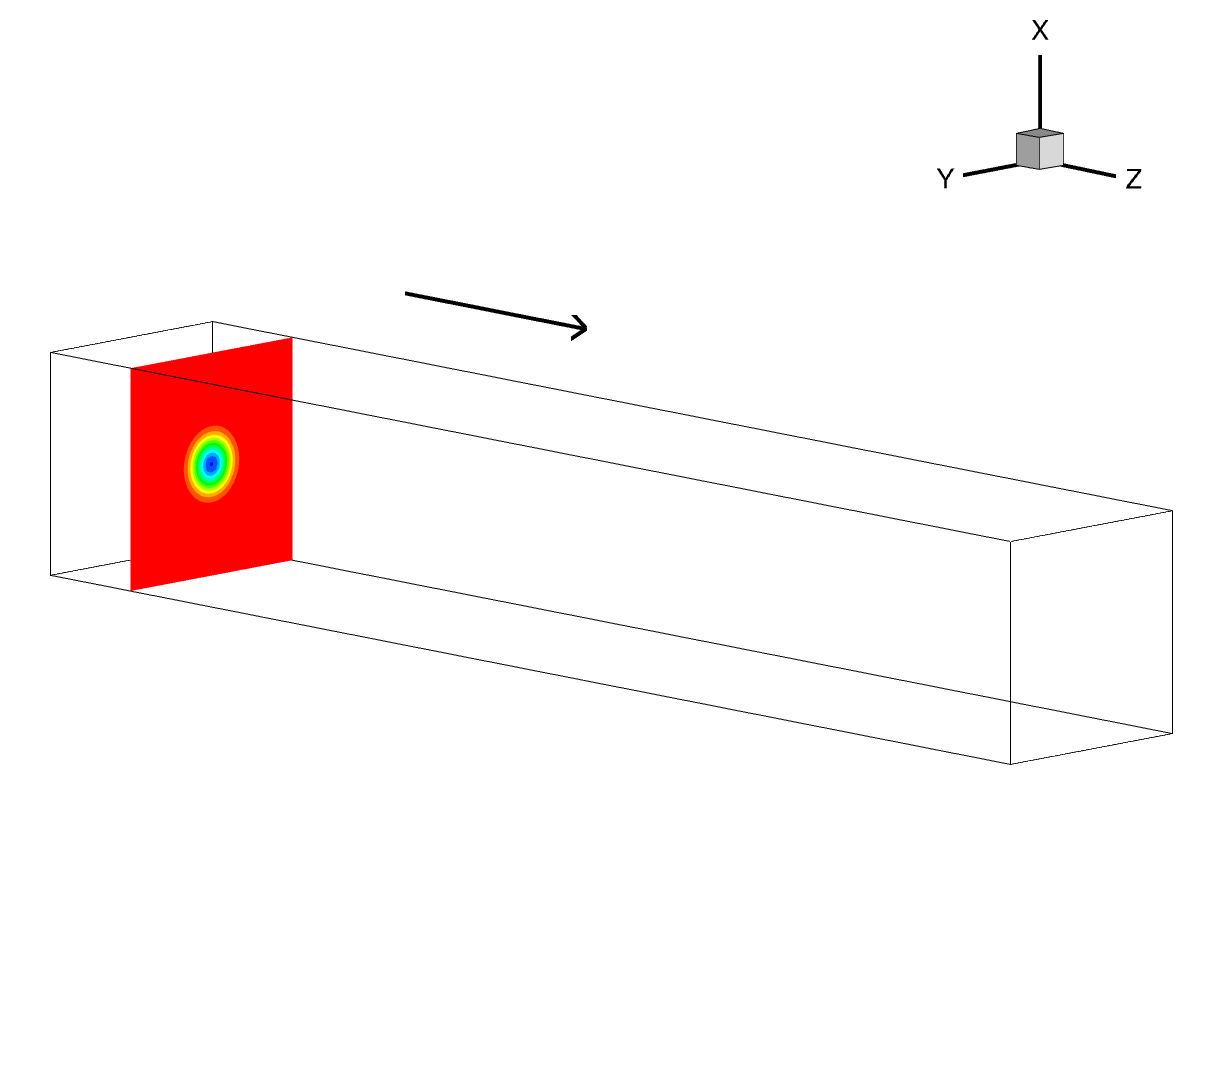
\includegraphics[clip=true, trim= 1.75cm 11.0cm 1.75cm 0.5cm,width=0.99\linewidth]{./figures/vortex3d/vortex3d}                  
     \caption{Illustration of the vortex advection.}
     \label{vortex3d}
\end{figure}
%%%%%%%%%%%%%%%%%%%%%%%%%%%%%%%%%%%
The geometry of the computational domain is a rectangular box, where $-5\le x \le5$, $-5\le y \le 5$, and $0\le z \le 12$. We demonstrate the ability of the schemes to preserve the vortex through a grid refinement study, where the coarse grid has dimensions $\Delta x=\Delta y=\Delta z=0.5$, the medium grid with $\Delta x=\Delta y=\Delta z=0.25$, and the fine grid with $\Delta x=\Delta y=\Delta z=0.125$. The time step is set to be $\Delta t=0.04$ and the final time is $t=10$. The test cases are simulated with the baseline MUSCL scheme, the original and the extended eddy-preserving limiter schemes. The computed results are denoted by ``MUSCL'', ``EDDY'', and ``EDDY-P'' respectively.
%%%%%%%%%%%%%%%%%%%%%%%%%%%%%%%%%%%%%%%%%%%%%%%%%%%%%%%%%%%%%%%%
\begin{figure*}[t]
\centering
     \subfigure[$t=2$ on coarse grid]{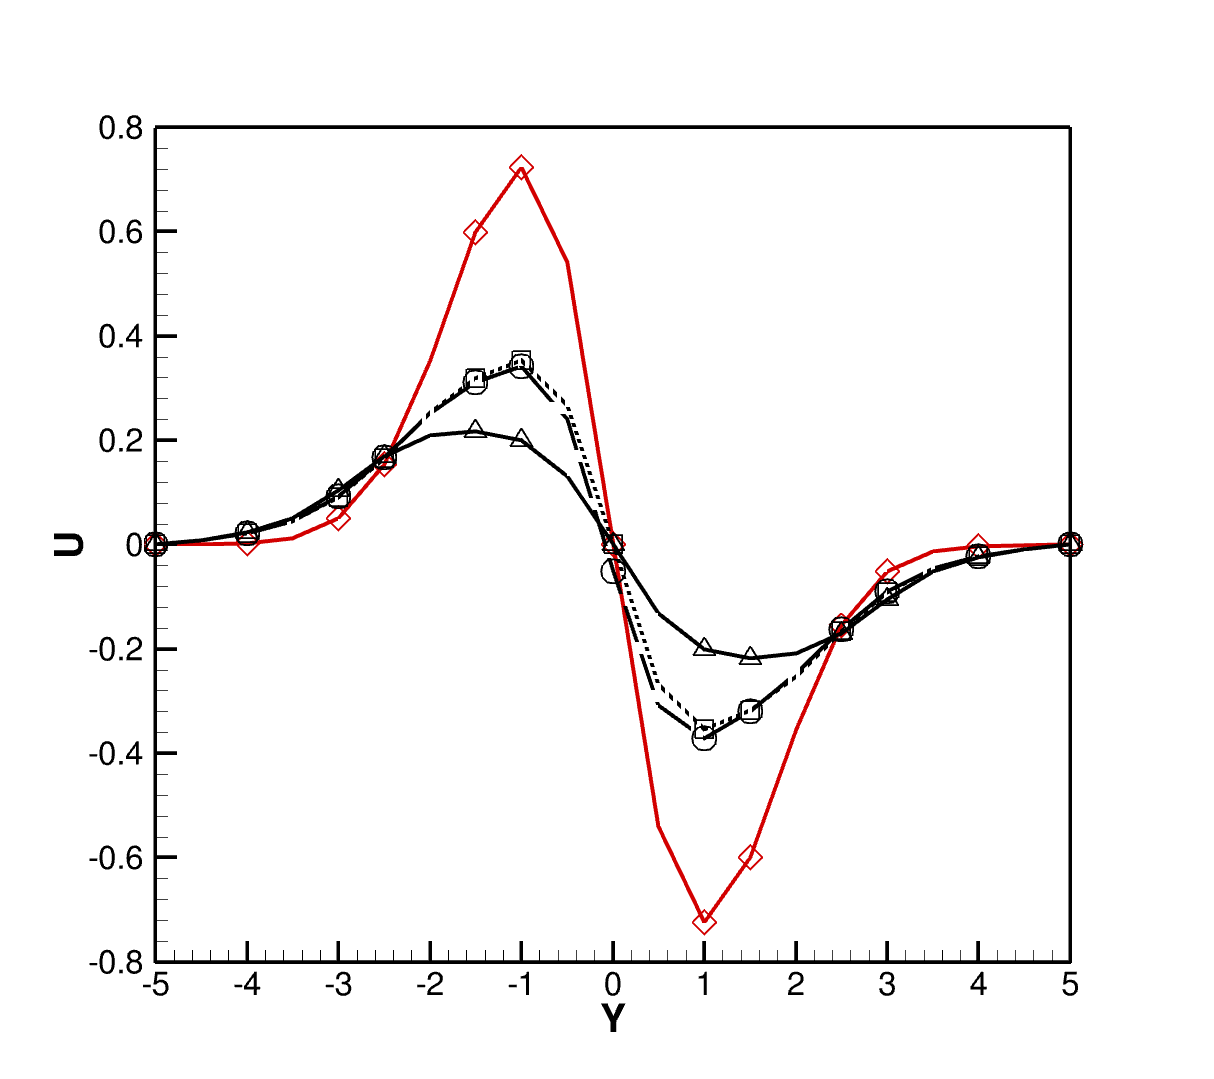
\includegraphics[clip=true, trim= 1.5cm 1.25cm 0.5cm 0.5cm,width=0.325\linewidth]{./figures/vortex3d/04up/04u1}}              
     \subfigure[$t=2$ on medium grid]{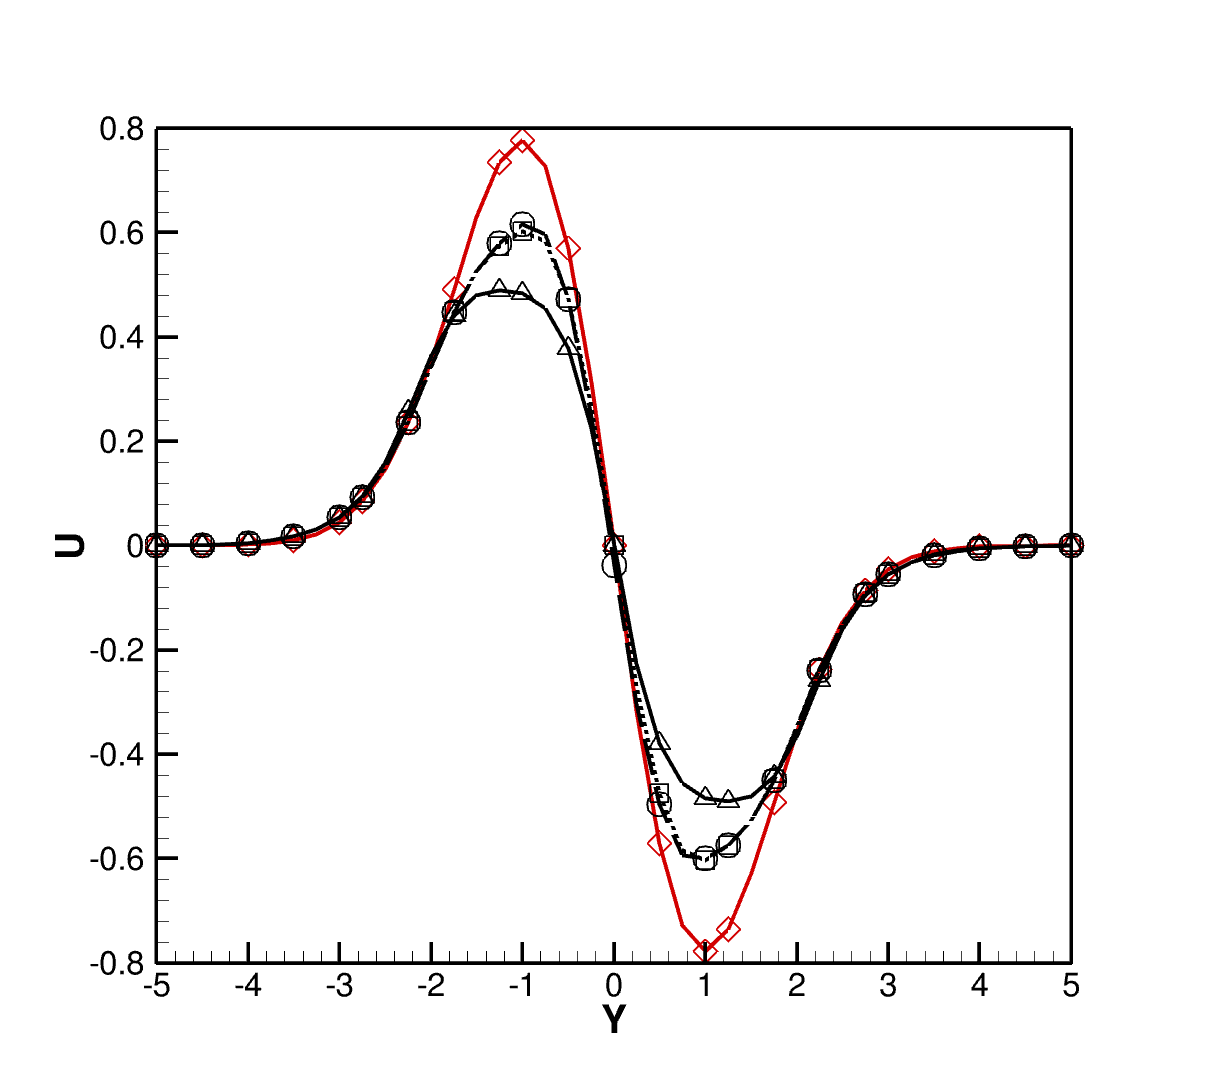
\includegraphics[clip=true, trim= 1.5cm 1.25cm 0.5cm 0.5cm,width=0.325\linewidth]{./figures/vortex3d/03up/03u1}}
     \subfigure[$t=2$ on fine grid]{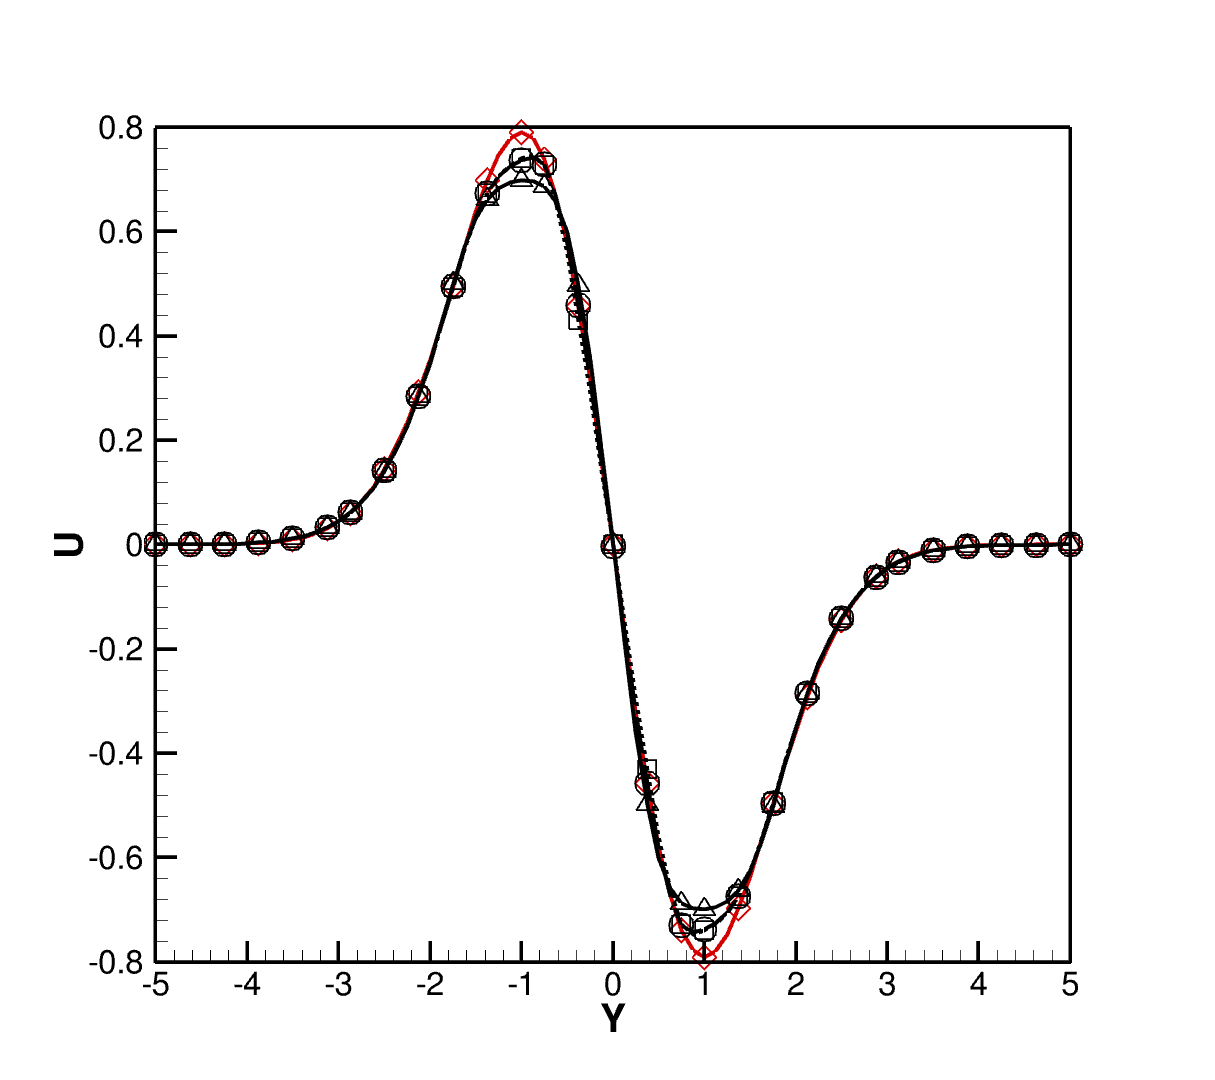
\includegraphics[clip=true, trim= 1.5cm 1.25cm 0.5cm 0.5cm,width=0.325\linewidth]{./figures/vortex3d/05up/05u1}}
     \subfigure[$t=6$ on coarse grid]{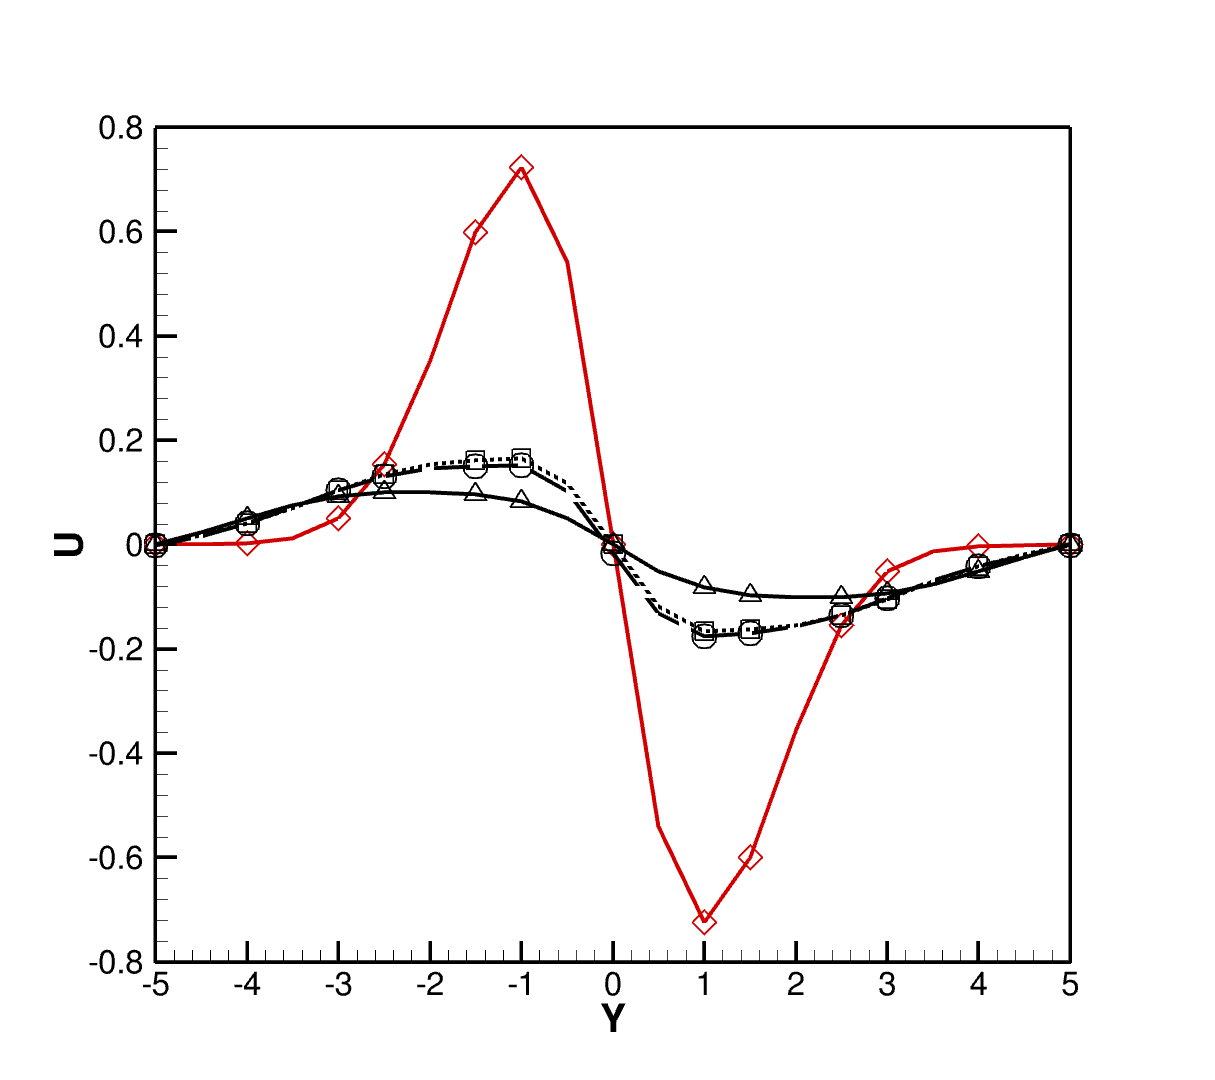
\includegraphics[clip=true, trim= 1.5cm 1.25cm 0.5cm 0.5cm,width=0.325\linewidth]{./figures/vortex3d/04up/04u3}}              
     \subfigure[$t=6$ on medium grid]{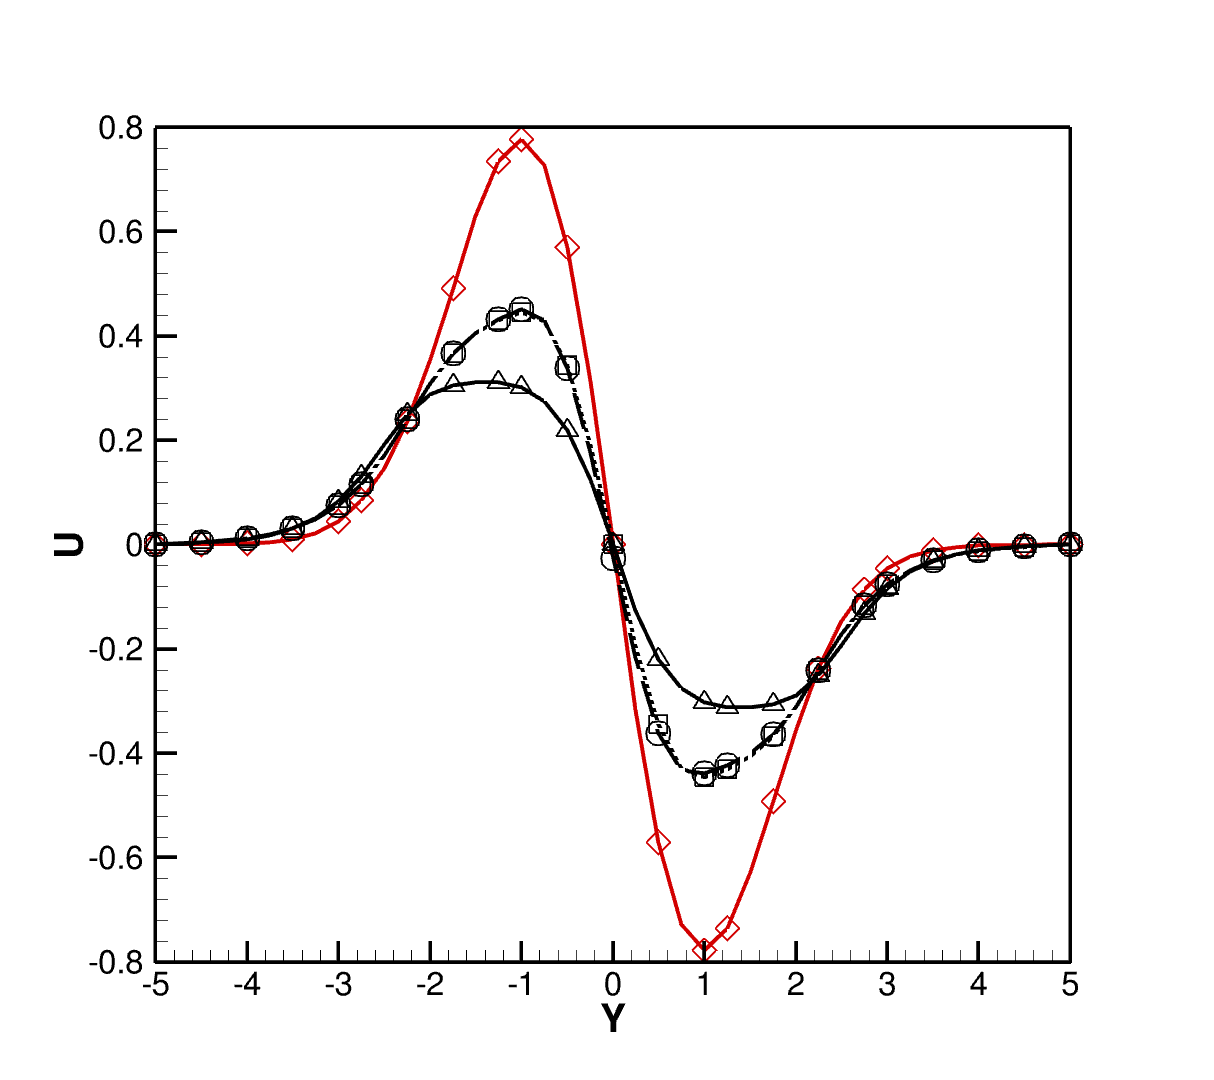
\includegraphics[clip=true, trim= 1.5cm 1.25cm 0.5cm 0.5cm,width=0.325\linewidth]{./figures/vortex3d/03up/03u3}}
     \subfigure[$t=6$ on fine grid]{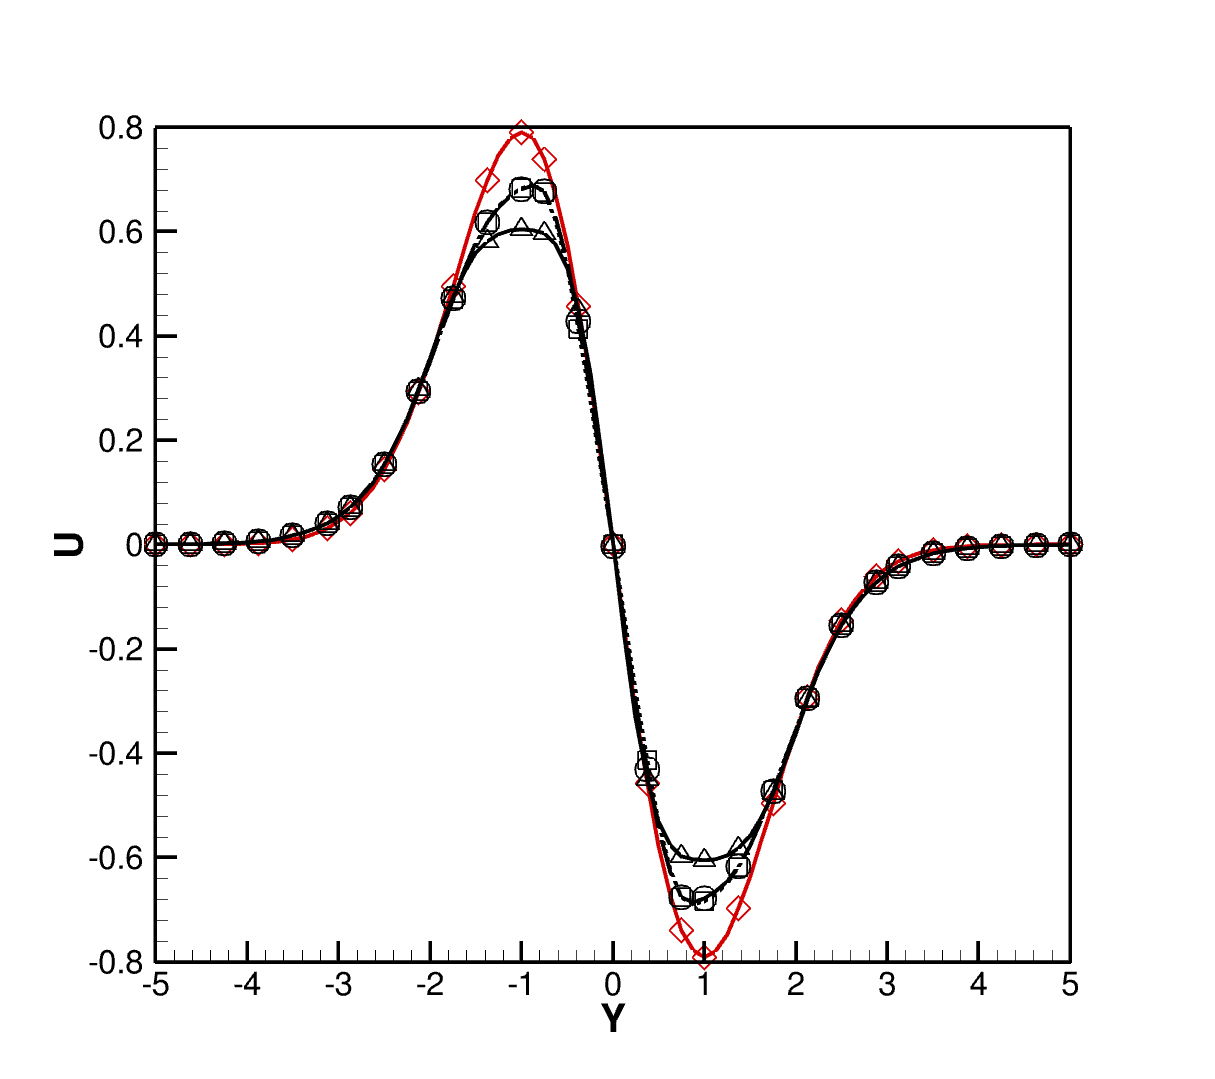
\includegraphics[clip=true, trim= 1.5cm 1.25cm 0.5cm 0.5cm,width=0.325\linewidth]{./figures/vortex3d/05up/05u3}}
     \subfigure[$t=10$ on coarse grid]{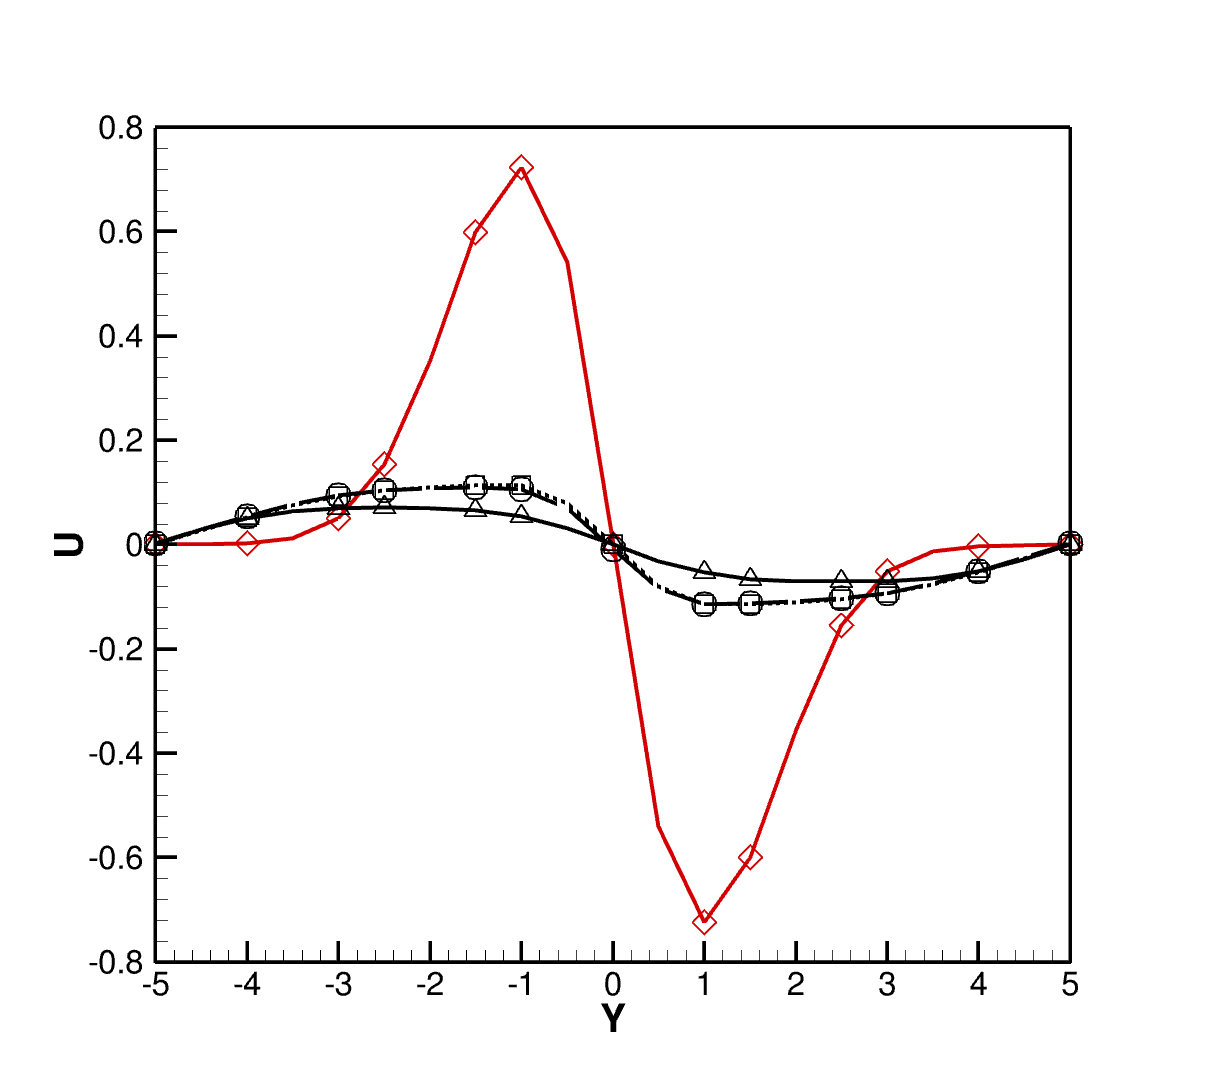
\includegraphics[clip=true, trim= 1.5cm 1.25cm 0.5cm 0.5cm,width=0.325\linewidth]{./figures/vortex3d/04up/04u5}}              
     \subfigure[$t=10$ on medium grid]{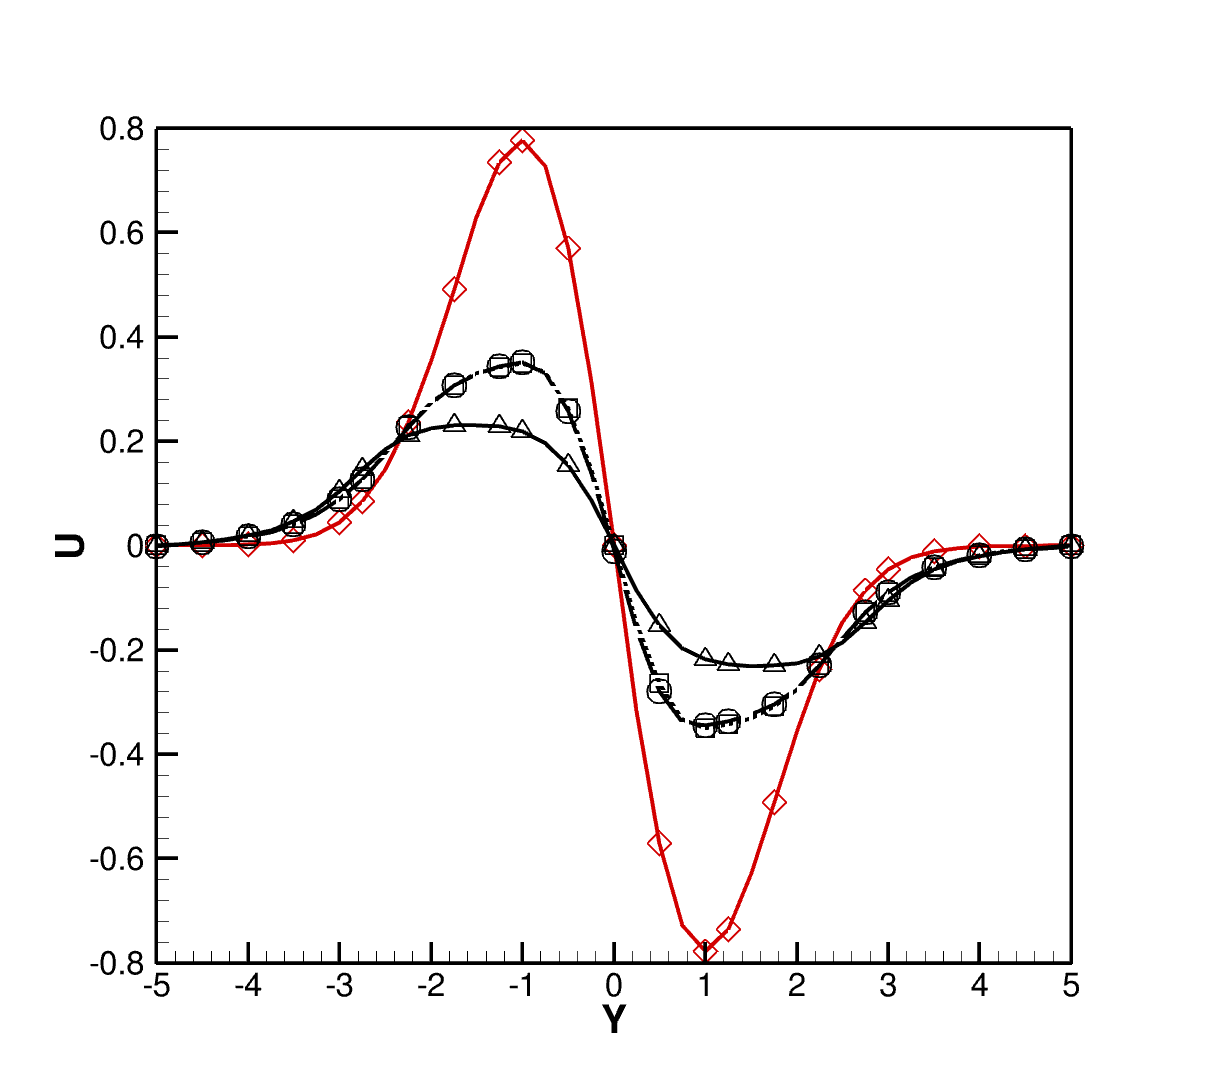
\includegraphics[clip=true, trim= 1.5cm 1.25cm 0.5cm 0.5cm,width=0.325\linewidth]{./figures/vortex3d/03up/03u5}}
     \subfigure[$t=10$ on fine grid]{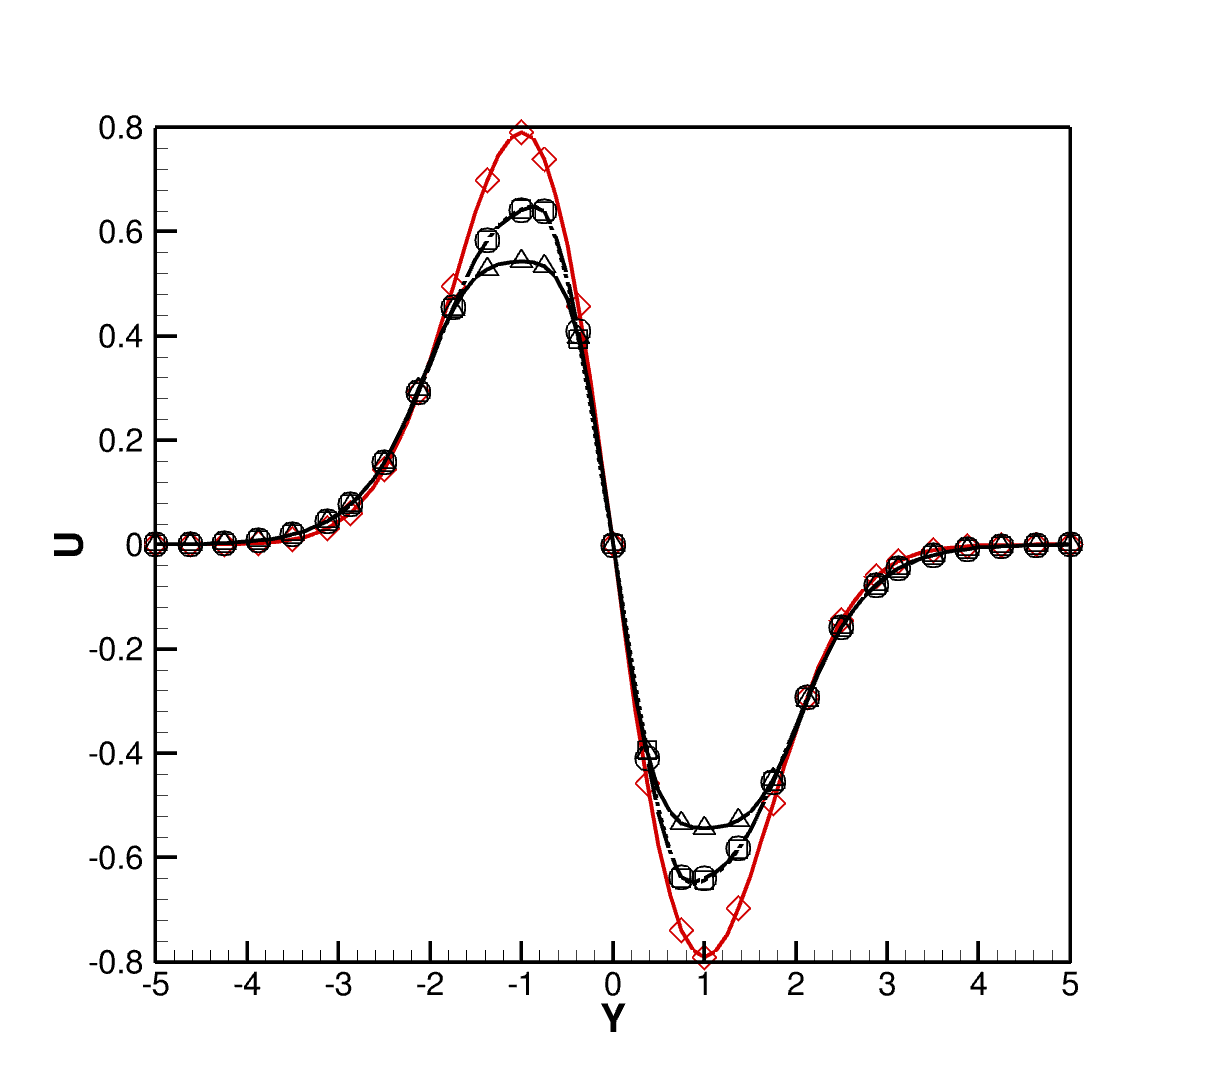
\includegraphics[clip=true, trim= 1.5cm 1.25cm 0.5cm 0.5cm,width=0.325\linewidth]{./figures/vortex3d/05up/05u5}}                   
     \caption{Velocity profiles at $x=0$. (MUSCL: \mline; EDDY: \eline; EDDY-P: \epline; Exact: \exact.)}     
     \label{u135}
\end{figure*}
%%%%%%%%%%%%%%%%%%%%%%%%%%%%%%%%%%%%%%%%%%%%%%%%%%%%%%%%%%%%%%%%
The profiles of the $x$ component of velocity at $x=0$ and several time instances $t=2$, $t=6$, and $t=10$ are shown in Fig.~\ref{u135}. The relative $L^{2}$ norms of the error are plotted in Fig.~\ref{l2} (a). The profiles computed by the EDDY and EDDY-P schemes are similar, and hence the modification for the interpolation of pressure has little impact on the velocity profiles. The predictions of both the EDDY and EDDY-P schemes agree better against the exact solutions when compared to the MUSCL scheme, due to their lower numerical dissipations.
%%%%%%%%%%%%%%%%%%%%%%%%%%%%%%%%%%%%%%%%%%%%%%%%%%%%%%%%%%%%%%%%
\begin{figure*}[t]  
\centering
     \subfigure[$t=2$ on coarse grid]{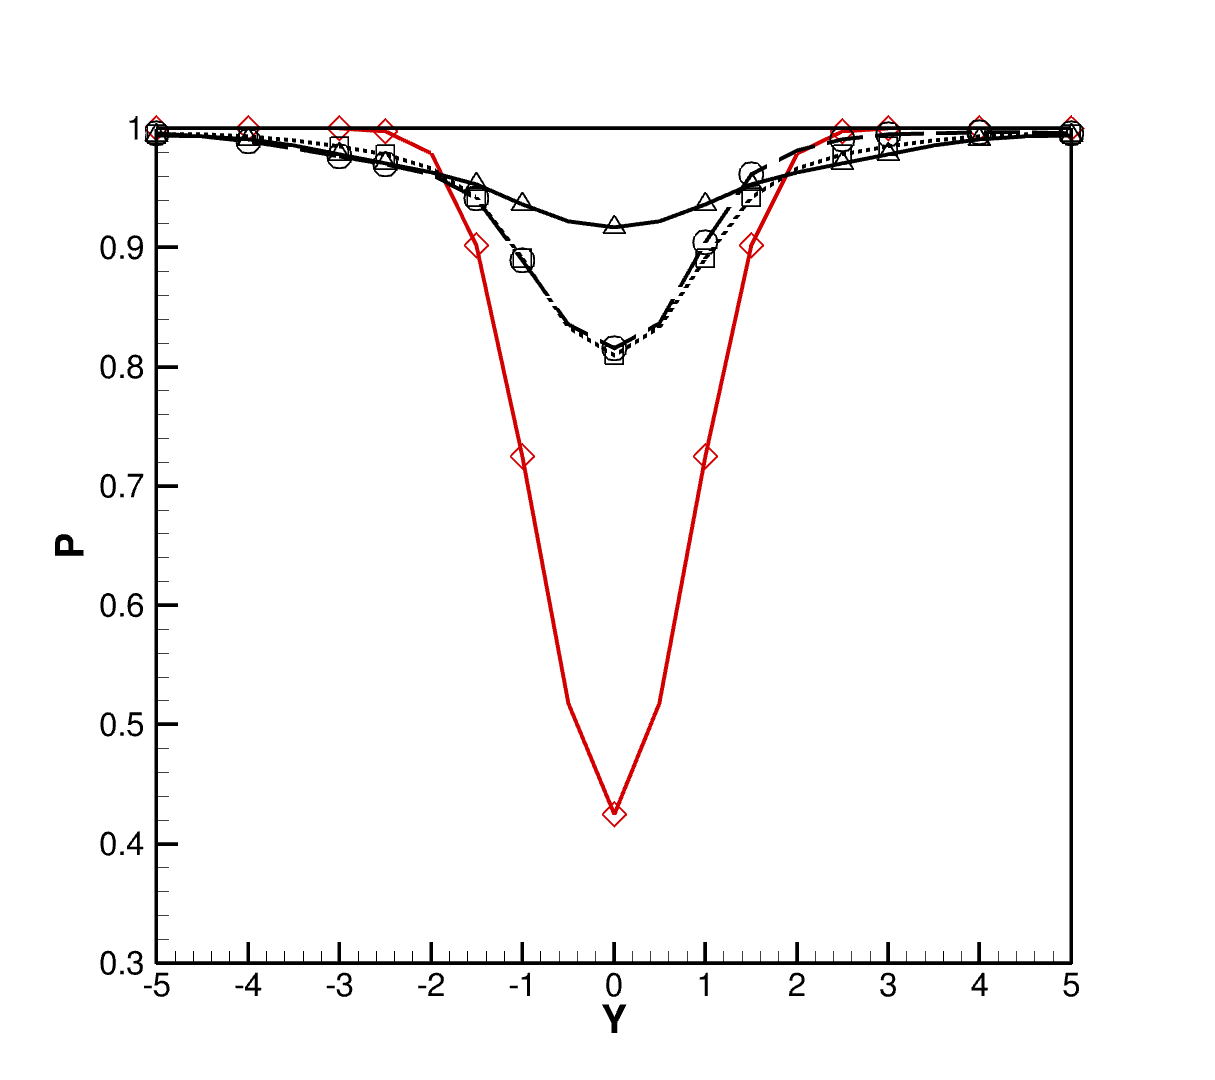
\includegraphics[clip=true, trim= 1.5cm 1.25cm 0.5cm 0.5cm,width=0.325\linewidth]{./figures/vortex3d/04up/04p1}}              
     \subfigure[$t=2$ on medium grid]{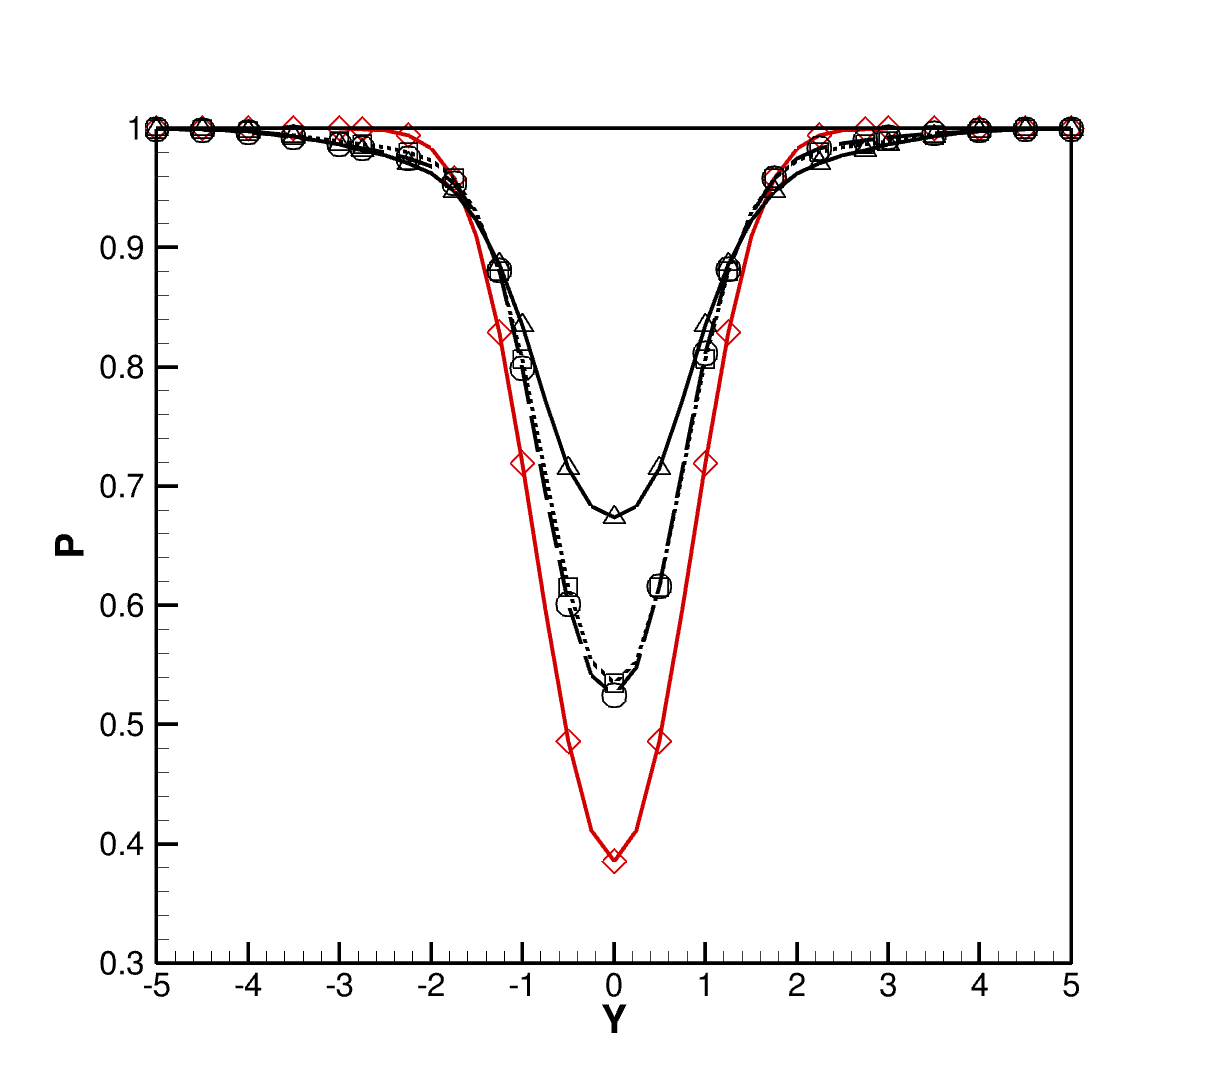
\includegraphics[clip=true, trim= 1.5cm 1.25cm 0.5cm 0.5cm,width=0.325\linewidth]{./figures/vortex3d/03up/03p1}}
     \subfigure[$t=2$ on fine grid]{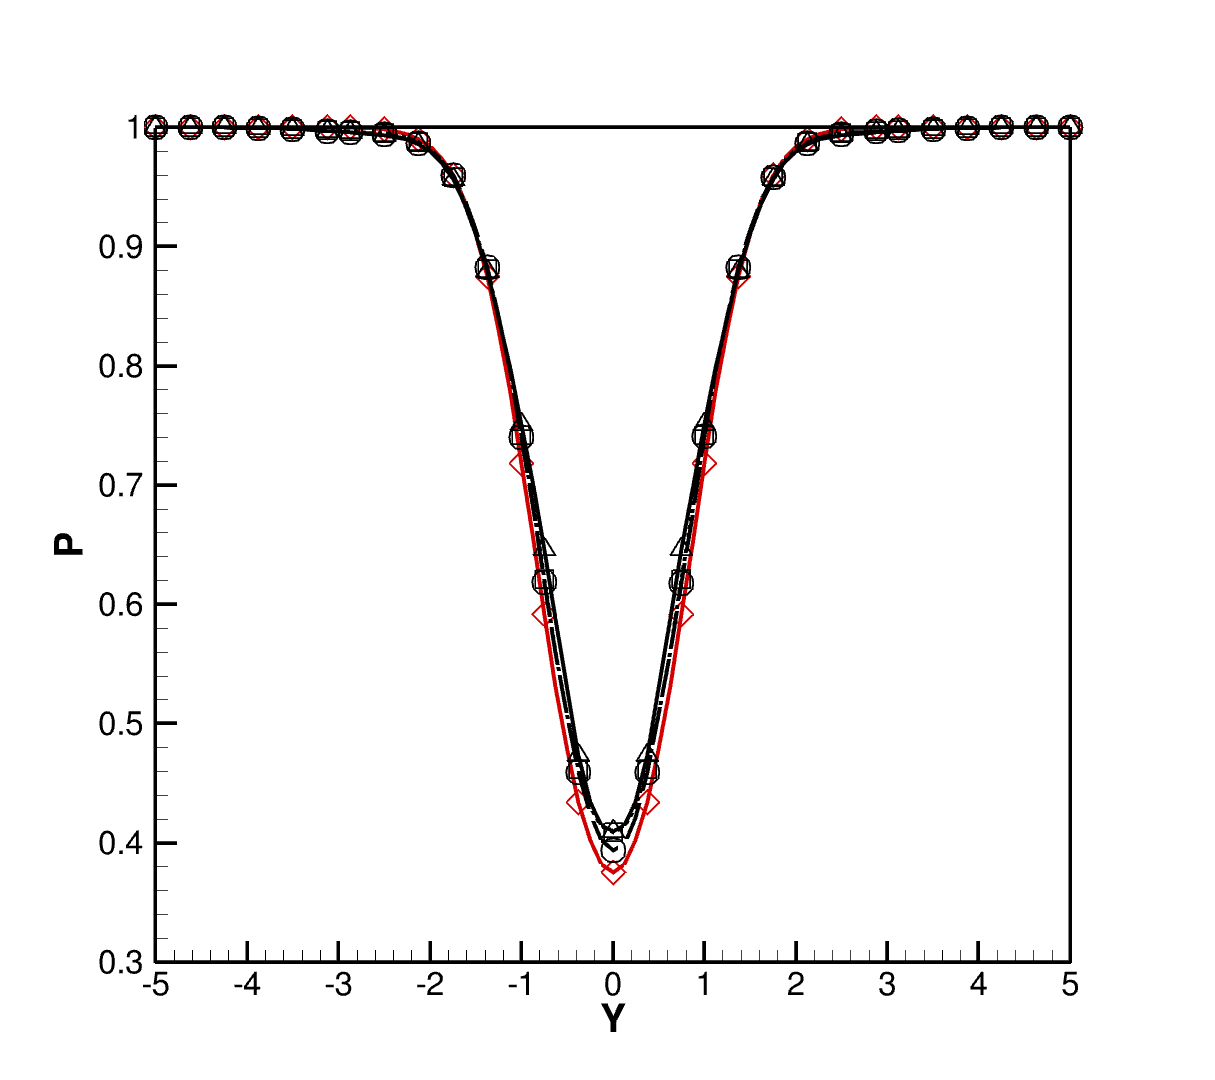
\includegraphics[clip=true, trim= 1.5cm 1.25cm 0.5cm 0.5cm,width=0.325\linewidth]{./figures/vortex3d/05up/05p1}}
     \subfigure[$t=6$ on coarse grid]{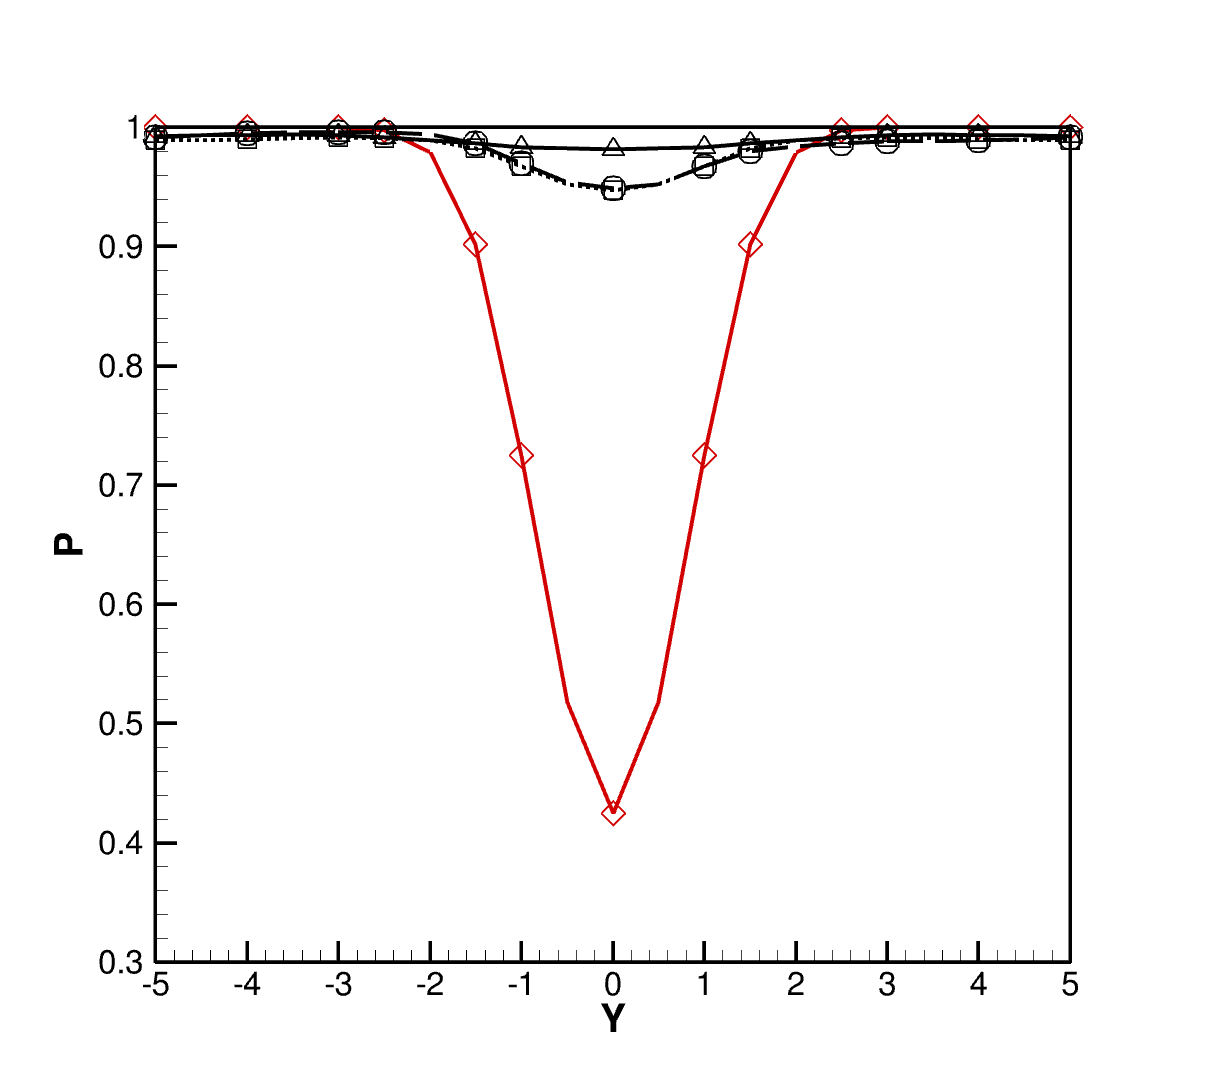
\includegraphics[clip=true, trim= 1.5cm 1.25cm 0.5cm 0.5cm,width=0.325\linewidth]{./figures/vortex3d/04up/04p3}}              
     \subfigure[$t=6$ on medium grid]{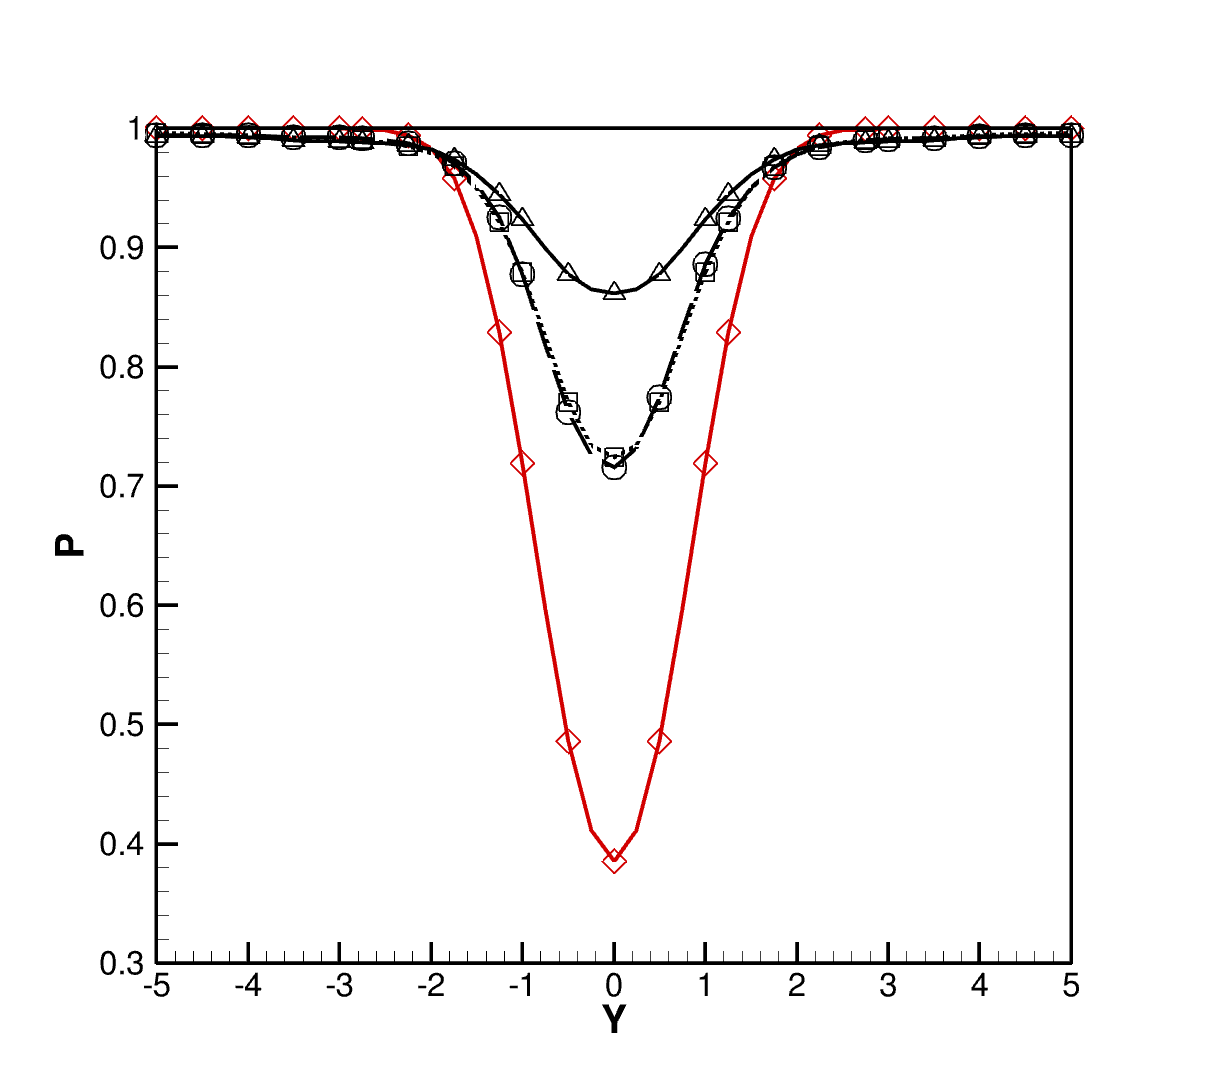
\includegraphics[clip=true, trim= 1.5cm 1.25cm 0.5cm 0.5cm,width=0.325\linewidth]{./figures/vortex3d/03up/03p3}}
     \subfigure[$t=6$ on fine grid]{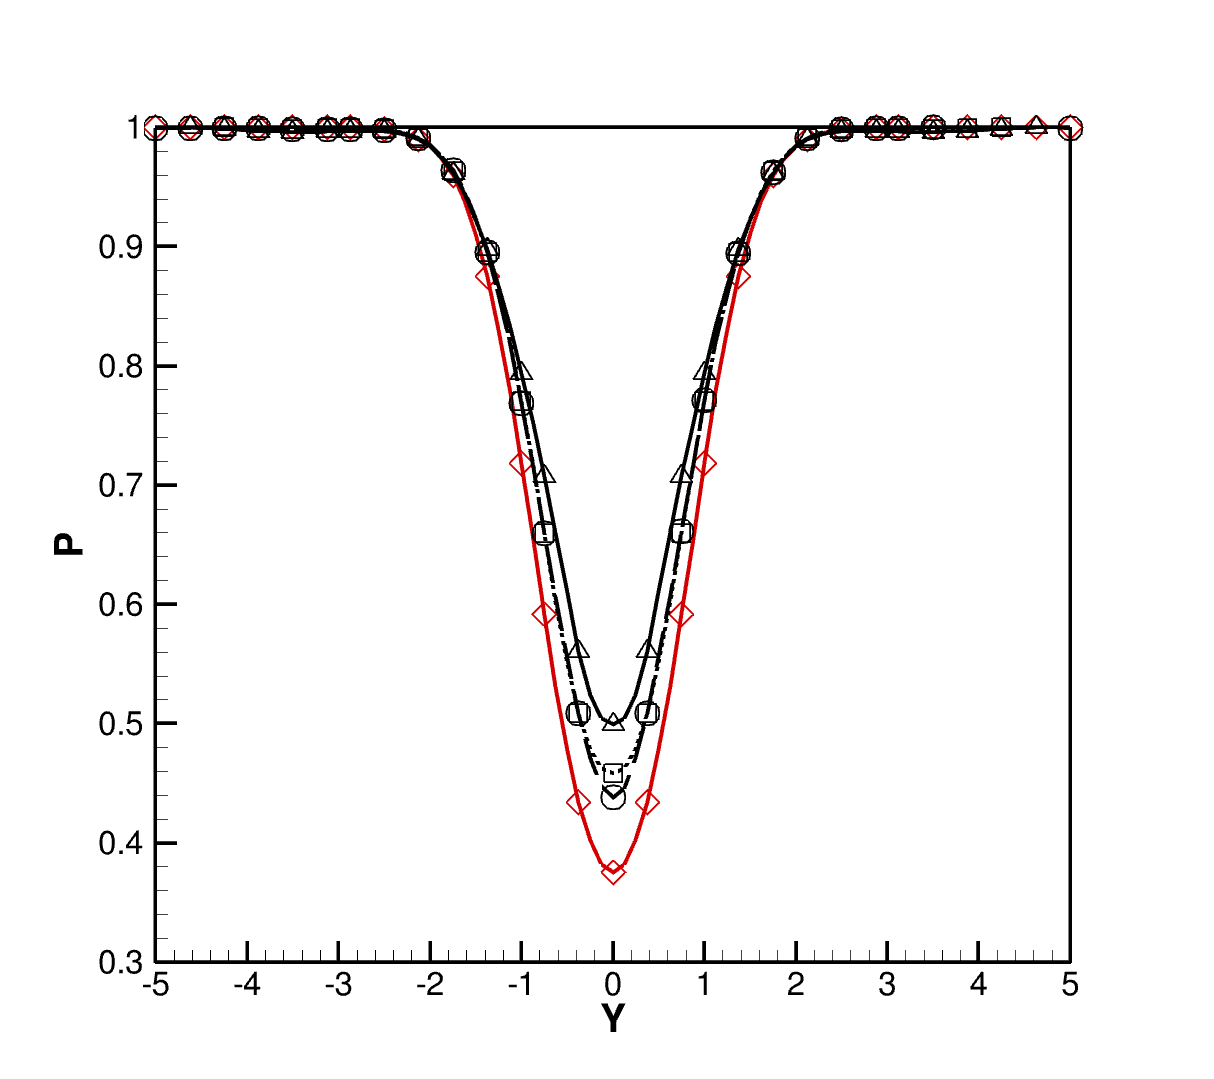
\includegraphics[clip=true, trim= 1.5cm 1.25cm 0.5cm 0.5cm,width=0.325\linewidth]{./figures/vortex3d/05up/05p3}}
     \subfigure[$t=10$ on coarse grid]{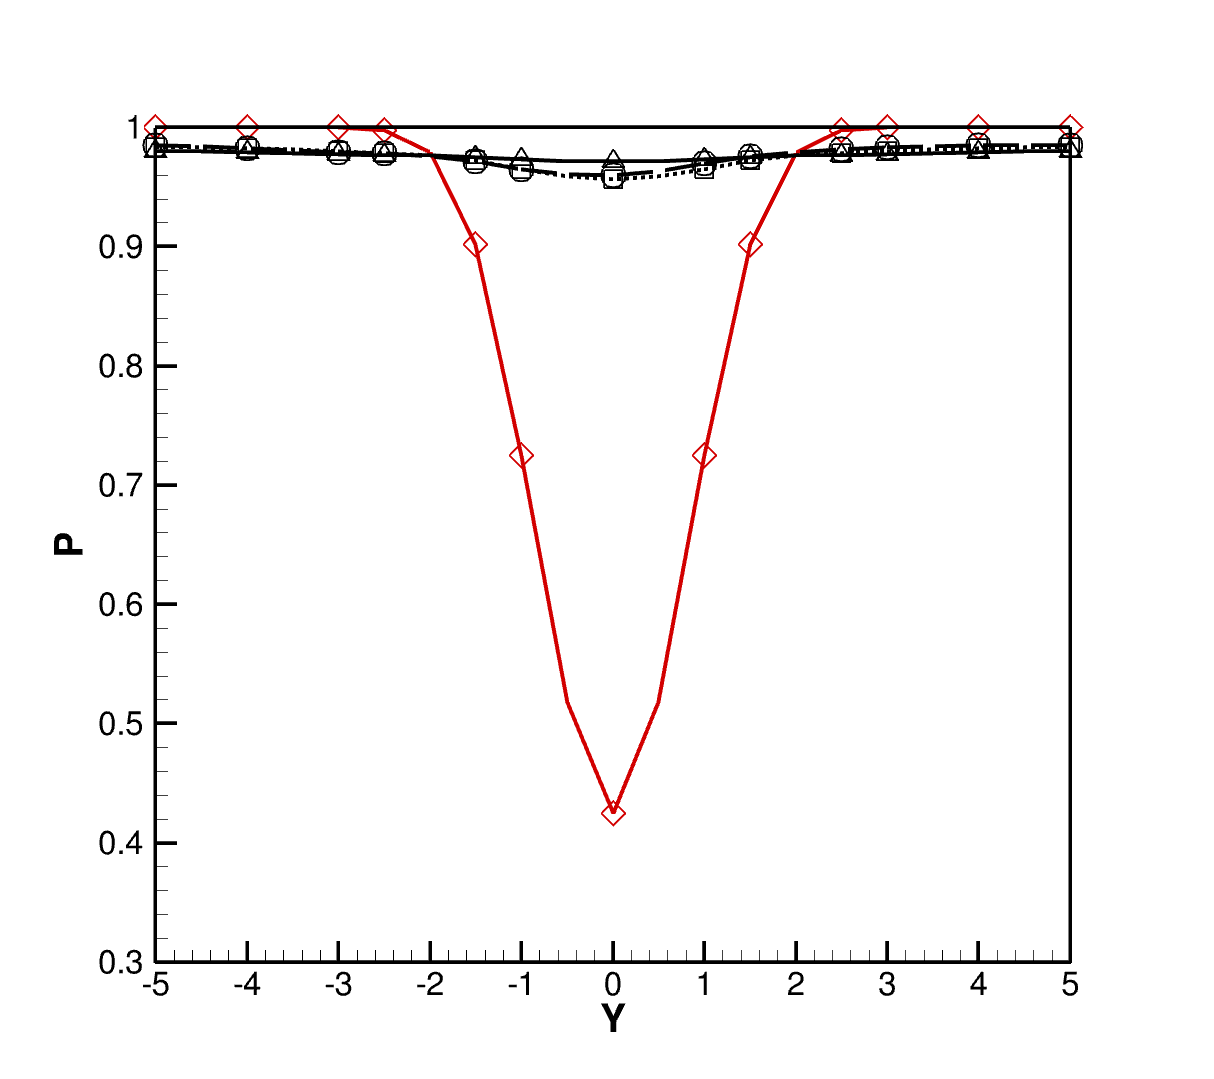
\includegraphics[clip=true, trim= 1.5cm 1.25cm 0.5cm 0.5cm,width=0.325\linewidth]{./figures/vortex3d/04up/04p5}}              
     \subfigure[$t=10$ on medium grid]{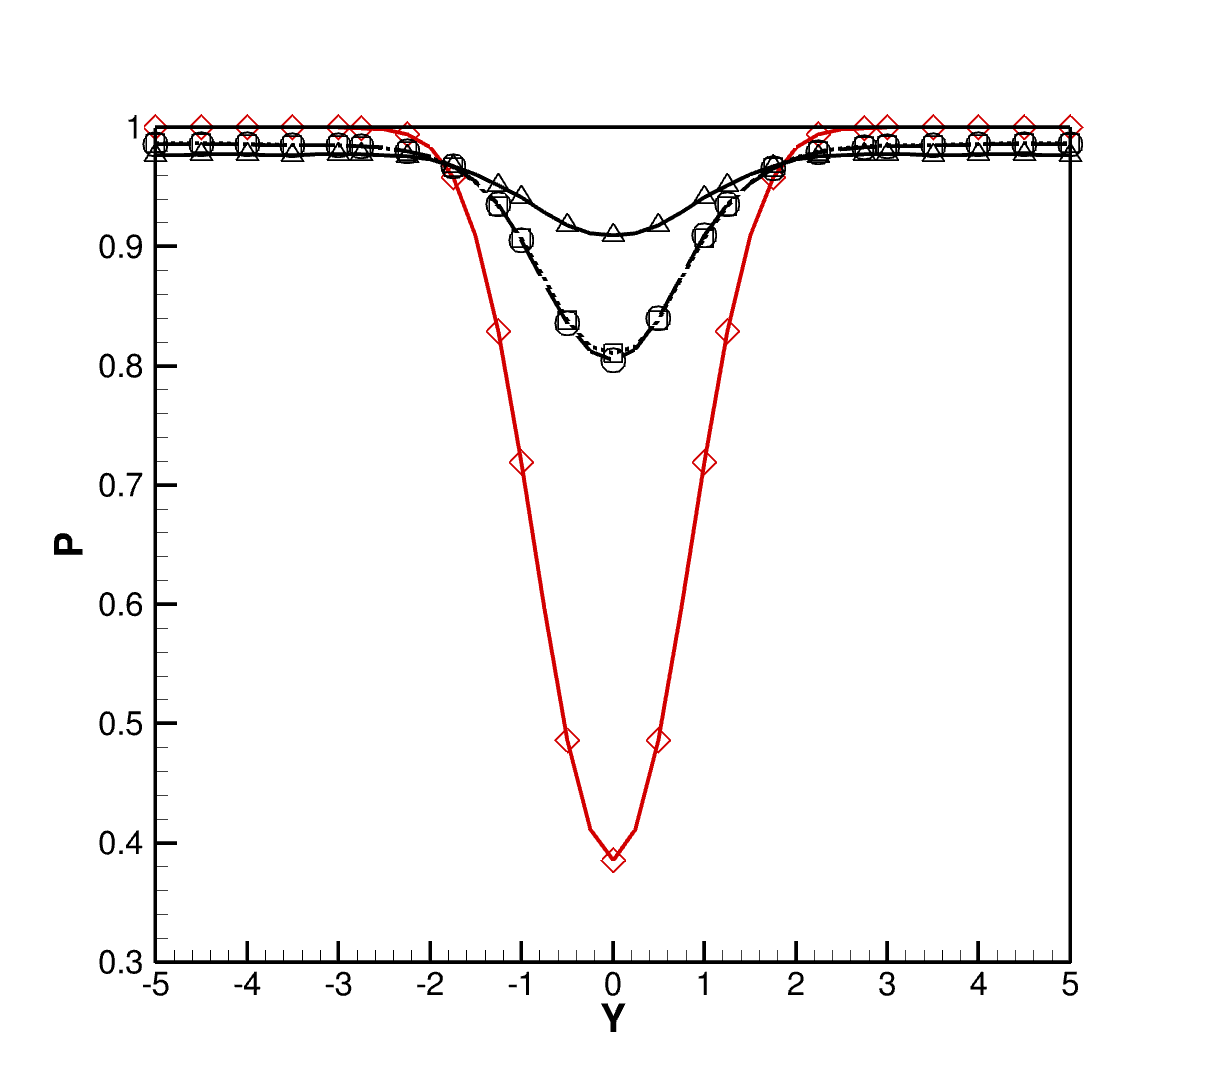
\includegraphics[clip=true, trim= 1.5cm 1.25cm 0.5cm 0.5cm,width=0.325\linewidth]{./figures/vortex3d/03up/03p5}}
     \subfigure[$t=10$ on fine grid]{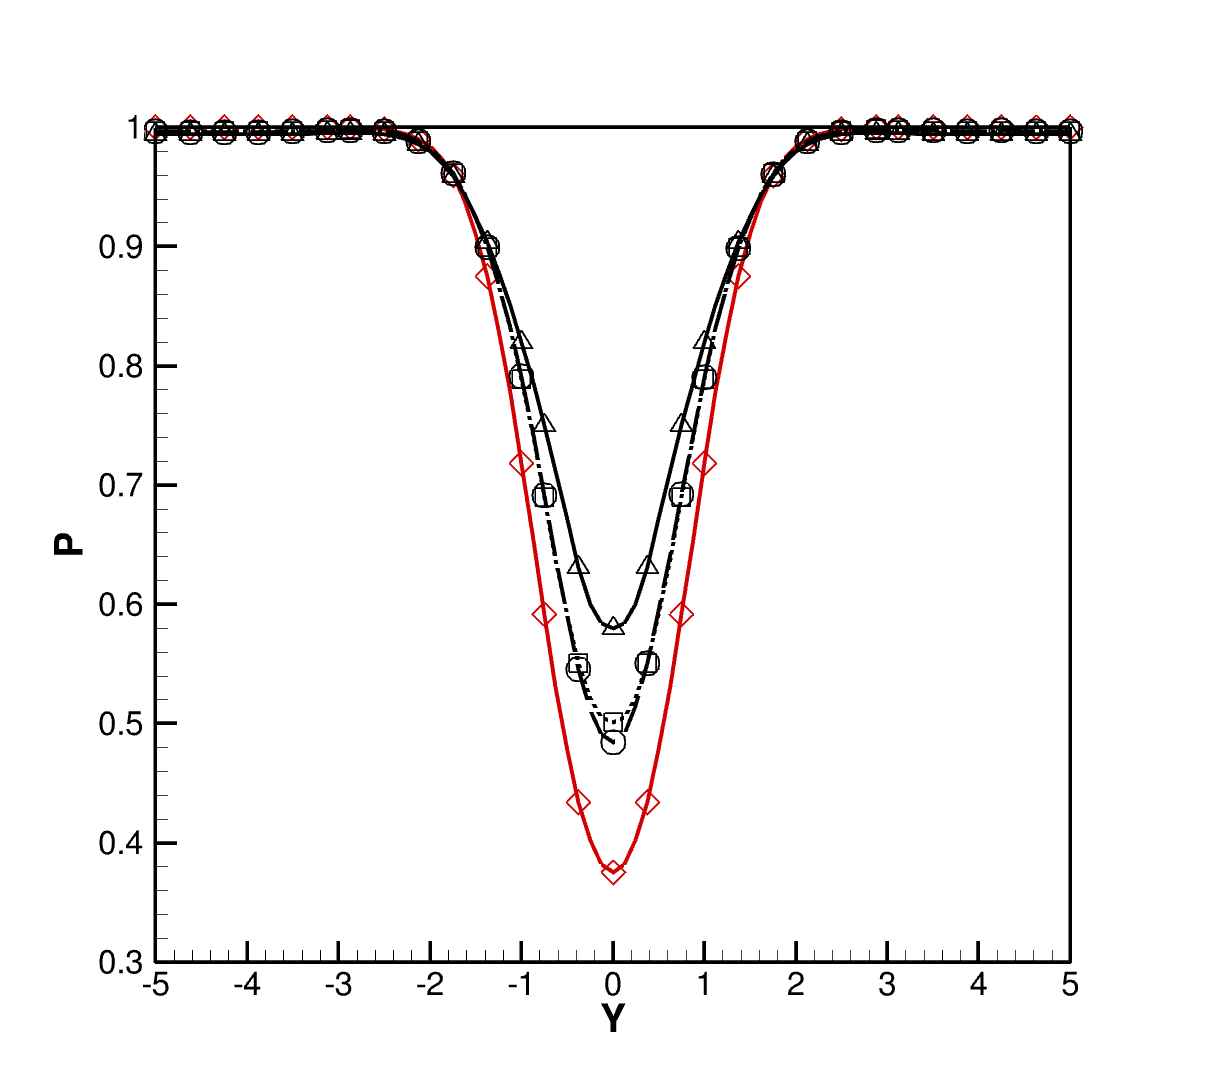
\includegraphics[clip=true, trim= 1.5cm 1.25cm 0.5cm 0.5cm,width=0.325\linewidth]{./figures/vortex3d/05up/05p5}}                   
     \caption{Pressure profiles at $x=0$. (MUSCL: \mline; EDDY: \eline; EDDY-P: \epline; Exact: \exact.)}     
     \label{p135}
\end{figure*}
%%%%%%%%%%%%%%%%%%%%%%%%%%%%%%%%%%%%%%%%%%%%%%%%%%%%%%%%%%%%%%%%
The pressure profiles at $x=0$ and several time instances $t=2$, $t=6$, and $t=10$ are shown in Fig.~\ref{p135}, while the relative $L^{2}$ norms of the error are plotted in Fig.~\ref{l2} (b). The EDDY scheme outperforms the MUSCL scheme, while the EDDY-P scheme demonstrates a slight further improvement, which shows that the modification for the interpolation of pressure is able to further reduce the dissipation. 


The vortex core regions on the medium grid for all schemes are represented by the contour lines of $Q=0$, as shown in Fig.~\ref{q}. As time advances, the vortex core of the MUSCL scheme grows, while that of the EDDY and EDDY-P are maintained, which demonstrates the schemes ability to preserve the vortex due to their lower dissipation.


A study of accuracy was performed for all three schemes on four consecutively refined grids. The $L^{2}$ error of pressure at $t=2$ with respect to the grid spacing is plotted in Fig.~\ref{order}. The slopes of all three schemes are able to match the slope of the referenced 2nd-order line as the grid is refined.
%%%%%%%%%%%%%%%%%%%%%%%%%%%%%%%%%%%%%%%%%%%%%%%%%%%%%%%%%%%%%%%%
\begin{figure}[t]  
\centering
     \subfigure[]{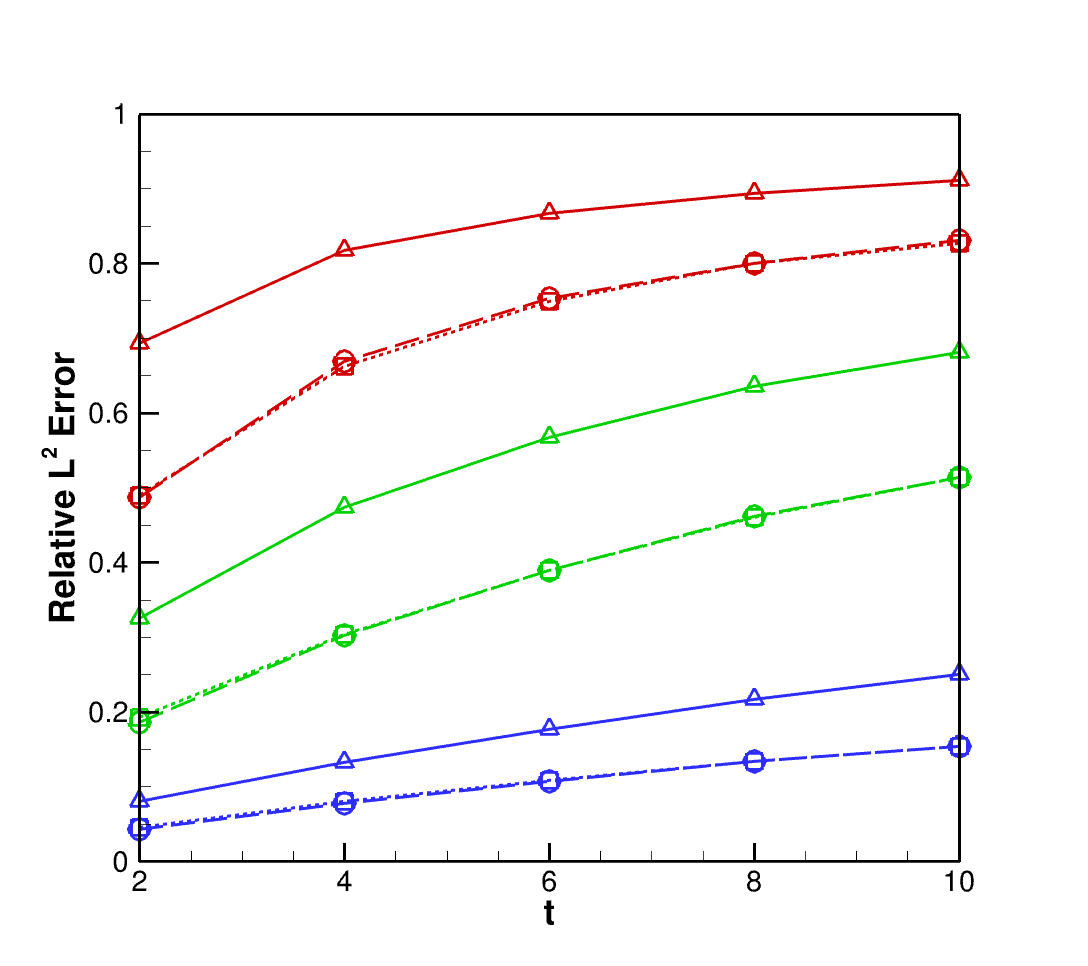
\includegraphics[clip=true, trim= 1.25cm 1.25cm 0.5cm 0.5cm,width=0.49\linewidth]{./figures/vortex3d/l2/u}}              
     \subfigure[]{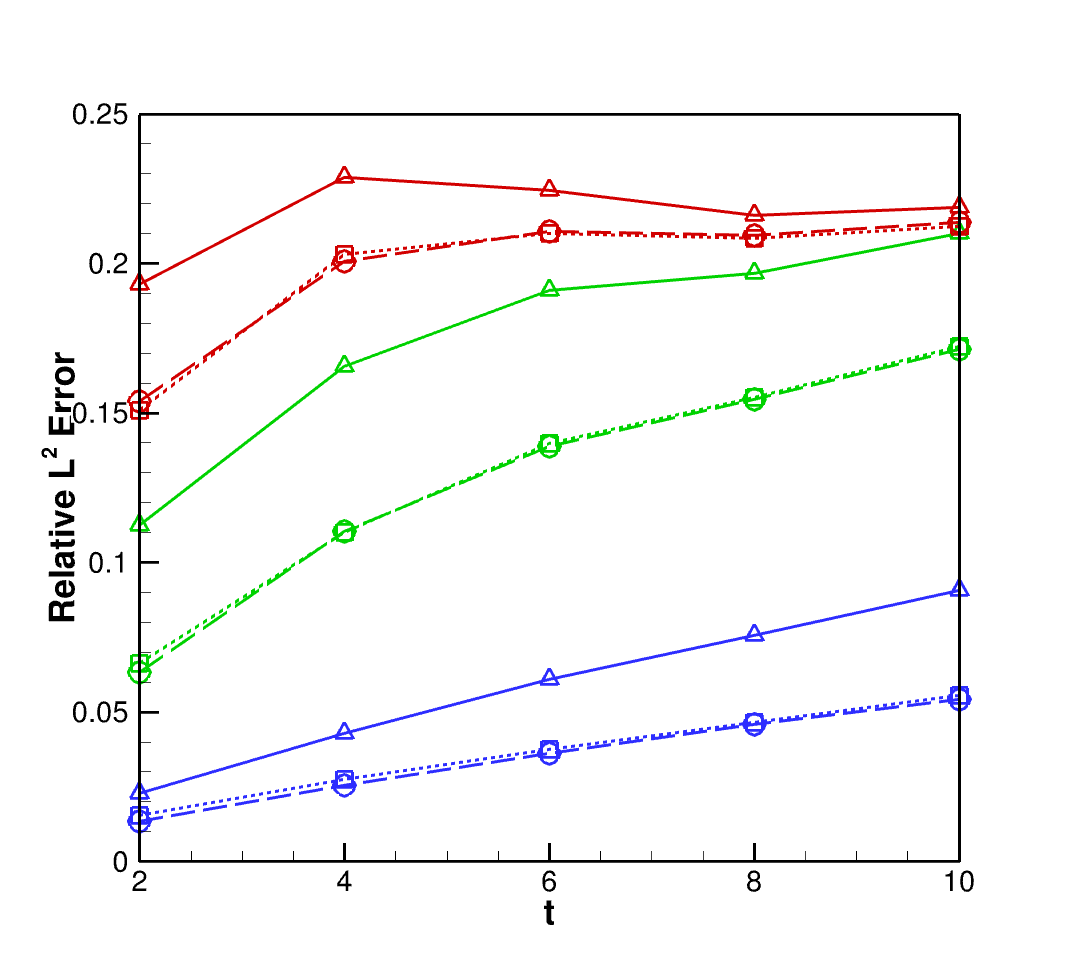
\includegraphics[clip=true, trim= 1.25cm 1.25cm 0.5cm 0.5cm,width=0.49\linewidth]{./figures/vortex3d/l2/p}}                 
     \caption{Relative $L^{2}$ error of (a)velocity (b)pressure. (Coarse grid: MUSCL: \mliner; EDDY: \eliner; EDDY-P: \epliner. Medium grid: MUSCL: \mlineg; EDDY: \elineg; EDDY-P: \eplineg. Fine grid: MUSCL: \mlineb; EDDY: \elineb; EDDY-P: \eplineb.)}
     \label{l2}   
\end{figure}
%%%%%%%%%%%%%%%%%%%%%%%%%%%%%%%%%%%%%%%%%%%%%%%%%%%%%%%%%%%%%%%%
%%%%%%%%%%%%%%%%%%%%%%%%%%%%%%%%%%%%%%%%%%%%%%%%%%%%%%%%%%%%%%%%
%%%%%%%%%%%%%%%%%%%%%%%%%%%%%%%%%%%%%%%%%%%%%%%%%%%%%%%%%%%%%%%%
%%%%%%%%%%%%%%%%%%%%%%%%%%%%%%%%%%%%%%%%%%%%%%%%%%%%%%%%%%%%%%%%
%%%%%%%%%%%%%%%%%%%%%%%%%%%%%%%%%%%%%%%%%%%%%%%%%%%%%%%%%%%%%%%%
%%%%%%%%%%%%%%%%%%%%%%%%%%%%%%%%%%%%%%%%%%%%%%%%%%%%%%%%%%%%%%%%
\begin{figure}[t]  
\centering
     \subfigure[]{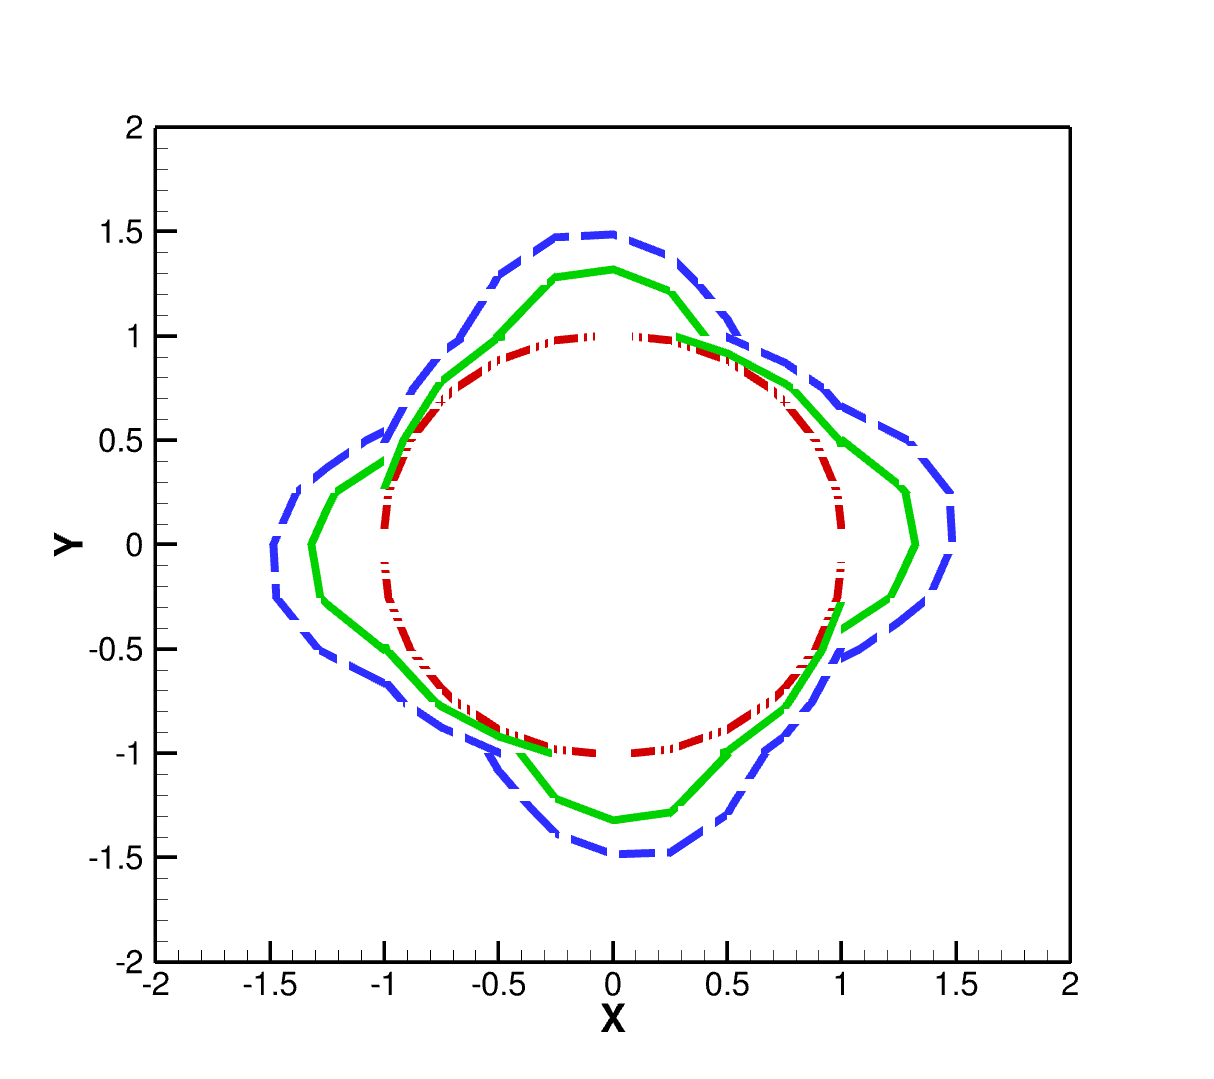
\includegraphics[clip=true, trim= 1.5cm 1.25cm 0.5cm 0.5cm,width=0.325\linewidth]{./figures/vortex3d/lines/m}}              
     \subfigure[]{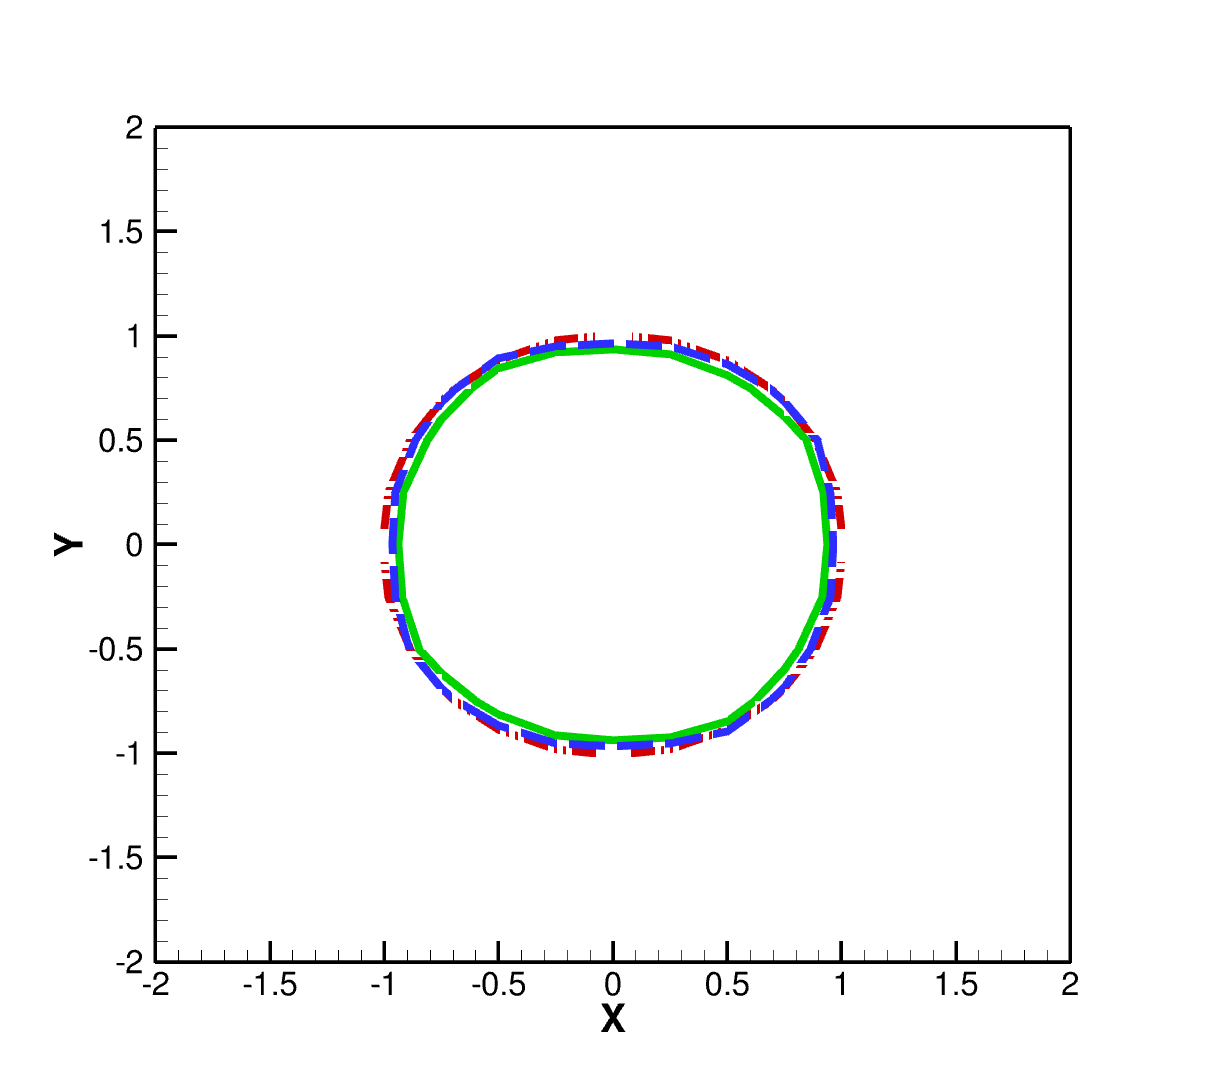
\includegraphics[clip=true, trim= 1.5cm 1.25cm 0.5cm 0.5cm,width=0.325\linewidth]{./figures/vortex3d/lines/e}}
     \subfigure[]{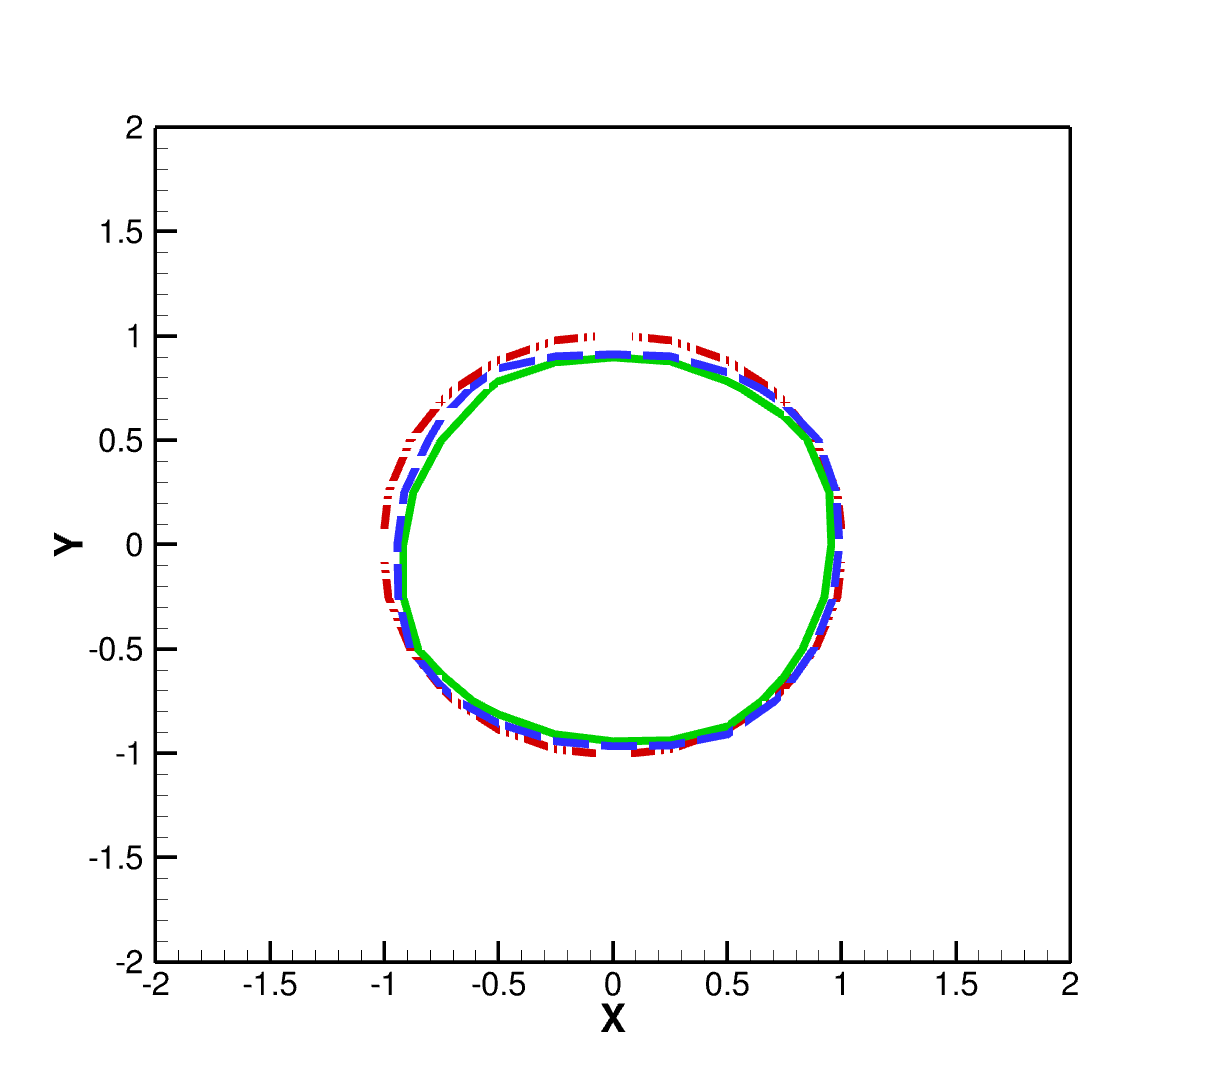
\includegraphics[clip=true, trim= 1.5cm 1.25cm 0.5cm 0.5cm,width=0.325\linewidth]{./figures/vortex3d/lines/ep}}                    
     \caption{$Q=0$ contour lines on medium grid for (a)MUSCL (b)EDDY (c)EDDY-P schemes. ($t=0$: \redline; $t=4$: \greenline; $t=8$: \blueline.)}
     \label{q}   
\end{figure}
%%%%%%%%%%%%%%%%%%%%%%%%%%%%%%%%%%%%%%%%%%%%%%%%%%%%%%%%%%%%%%%%
%%%%%%%%%%%%%%%%%%%%%%%%%%%%%%%%%%%%%%%%%%%%%%%%%%%%%%%%%%%%%%%%
%%%%%%%%%%%%%%%%%%%%%%%%%%%%%%%%%%%%%%%%%%%%%%%%%%%%%%%%%%%%%%%%
\begin{figure}[t]  
\centering
     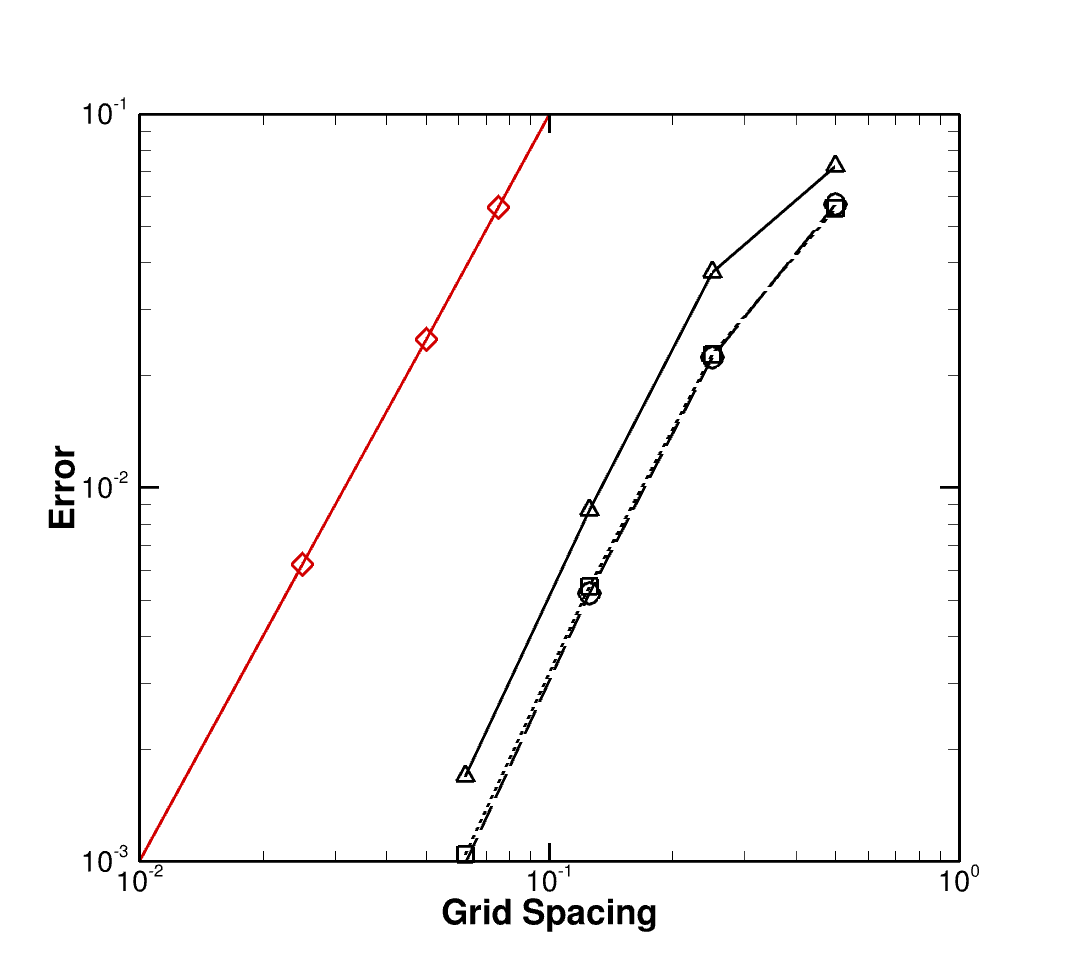
\includegraphics[clip=true, trim= 1.5cm 1.25cm 0.5cm 0.5cm,width=0.99\linewidth]{./figures/vortex3d/order}                            
     \caption{Accuracy study of different schemes. (MUSCL: \mline; EDDY: \eline; EDDY-P: \epline; 2nd-order: \exact.)}
     \label{order}   
\end{figure}













